\documentclass{article}
\usepackage{indentfirst}
\usepackage{multirow}\usepackage{makecell}\usepackage{diagbox}
\setlength{\parindent}{2em}
\usepackage{xeCJK}\usepackage{float}
\usepackage{xcolor}\usepackage{tcolorbox}
\usepackage{colortbl}
\usepackage{graphicx}
\usepackage{subfig}
\setCJKmainfont{SimSun} 
\usepackage{tikz}    
\usetikzlibrary{shapes.geometric,arrows.meta}        % 添加 TikZ 包以支持 tikzpicture 环境
\usepackage{pgfplots}        % 核心绘图包
\usepgfplotslibrary{patchplots}
\pgfplotsset{compat=1.17}
\usepackage{amsmath}
\usetikzlibrary{calc}
\usepackage{amssymb}
\usepackage{amsthm}
\usepackage{geometry}
\usepackage{tocbibind}
\usepackage{hyperref}
\usepackage{enumitem}
\geometry{a4paper,margin=2.5cm}
\usetikzlibrary{angles, quotes}
\usetikzlibrary{arrows.meta,calc}

\title{解析几何复习学案(天津专用)}
\author{小白高考数学}
\date{}

\hypersetup{
    colorlinks=true,    % 链接文字上色（false则加边框）
    linkcolor=black,     % 目录跳转链接颜色（黑色）
    urlcolor=blue,      % 网址链接颜色
    citecolor=green,    % 引用链接颜色
    bookmarks=true,     % 生成PDF书签（侧边栏）
    bookmarksnumbered=true, % 书签显示章节号
    pdfstartview=FitH   % PDF打开时自适应宽度
}

\renewcommand{\contentsname}{目录}
\begin{document}
\maketitle

\vspace{30\baselineskip}
\begin{center}
在数学的天地里，重要的不是我们知道什么，而是我们怎么知道什么
\end{center}
\begin{flushright}
    \rightskip=7em 
——毕达哥拉斯
\end{flushright}    
\newpage
\tableofcontents % 核心命令：生成目录
\newpage 

\section{知识要点}

\subsection{直线}

\vspace{1\baselineskip}

\textcolor{blue}{知识点1.}直线的倾斜角与斜率的关系：
\begin{center}
\begin{tabular}{|c|c|c|c|c|}
\hline
$\alpha$ 的大小 & $0^\circ$ & $0^\circ < \alpha < 90^\circ$ & $90^\circ$ & $90^\circ < \alpha < 180^\circ$ \\
\hline
$k$ 的范围 & $k=0$ & $k>0$ & 不存在 & $k<0$ \\
\hline
$k$ 的增减性 & \diagbox{}{} & \makecell{随 $\alpha$ 的增大\\而增大} & \diagbox{}{} & \makecell{随 $\alpha$ 的增大\\而增大} \\
\hline
\end{tabular}
\end{center}

\vspace{1em}

\textbf{注意} ： 下面特殊角的正切值要熟记：

\vspace{1em}

\begin{center}
\begin{tabular}{|c|c|c|c|c|c|c|c|}
\hline
倾斜角 \(\alpha\) & \(0^\circ\) & \(30^\circ\) & \(45^\circ\) & \(60^\circ\) & \(120^\circ\) & \(135^\circ\) & \(150^\circ\) \\
\hline
斜率 \(k\) & \(0\) & \(\dfrac{\sqrt{3}}{3}\) & \(1\) & \(\sqrt{3}\) & \(-\sqrt{3}\) & \(-1\) & \(-\dfrac{\sqrt{3}}{3}\) \\
\hline
\end{tabular}
\end{center}
\vspace{1\baselineskip}

\textcolor{blue}{知识点2.}经过两点 \(P_1(x_1, y_1)\), \(P_2(x_2, y_2)\) (\(x_1 \neq x_2\)) 的直线的斜率公式为
\[
k = \frac{y_2 - y_1}{x_2 - x_1}.
\]

\begin{tcolorbox}[colback=blue!10,colframe=blue!70!black,title=]
我们知道, 直线 \(P_1P_2\) 上的向量 \(\overrightarrow{P_1P_2}\) 以及与它平行的向量都是直线的方向向量, 直线 \(P_1P_2\) 的方向向量 \(\overrightarrow{P_1P_2}\) 的坐标为 \((x_2 - x_1, y_2 - y_1)\)。

当直线 \(P_1P_2\) 与 \(x\) 轴不垂直时, \(x_1 \neq x_2\), 此时向量 \(\frac{1}{x_2 - x_1}\overrightarrow{P_1P_2}\) 也是直线 \(P_1P_2\) 的方向向量, 且它的坐标为
\[
\frac{1}{x_2 - x_1}(x_2 - x_1, y_2 - y_1) = \left(1, \frac{y_2 - y_1}{x_2 - x_1}\right) = (1, k),
\]
其中 \(k\) 是直线 \(P_1P_2\) 的斜率。

因此, 若直线 \(l\) 的斜率为 \(k\), 它的一个方向向量的坐标为 \((x, y)\), 则
\[
k = \frac{y}{x}.
\]
\end{tcolorbox}
\vspace{1\baselineskip}

\textcolor{blue}{知识点3.}两条直线平行与垂直的判定

\subsection*{两条直线平行的判定}
\begin{enumerate}
    \item 特殊情况：若两条不重合的直线中一条没有斜率，另一条也没有斜率（即倾斜角均为 \(90^\circ\)），则两直线互相平行。
    \item 一般情况：对于斜率分别为 \(k_1, k_2\) 的两条直线 \(l_1, l_2\)，有
    \[
    l_1 \parallel l_2 \iff k_1 = k_2
    \]
    （前提：两条直线的斜率都存在）。
\end{enumerate}

\subsubsection*{特别提醒}
\begin{enumerate}
    \item \(l_1 \parallel l_2 \implies k_1 = k_2\)，或两条直线的斜率都不存在。
    \item 若直线 \(l_1, l_2\) 重合，仍有 \(k_1 = k_2\) 或斜率都不存在，此结论常用于用斜率证明三点共线。
\end{enumerate}

\subsection*{两条直线垂直的判定}
\begin{enumerate}
    \item 特殊情况：若两条直线中一条没有斜率（倾斜角为 \(90^\circ\)），另一条斜率为 \(0\)（倾斜角为 \(0^\circ\)），则两直线互相垂直。
    \item 一般情况：设两条直线的斜率分别为 \(k_1, k_2\)，则
    \[
    l_1 \perp l_2 \iff k_1 k_2 = -1
    \]
    （前提：两条直线的斜率都存在）。
\end{enumerate}
\vspace{1\baselineskip}

\textcolor{blue}{知识点4.}直线的表达式

\begin{table}[htbp]
  \centering
  % 调整表格列宽，适配参数方程的较长公式
  \begin{tabular}{|m{1.5cm}|m{4.5cm}|m{4.5cm}|m{3cm}|}
    \hline
    方程形式 & 方程 & 常数的几何意义 & 适用条件 \\
    \hline
    点斜式 & \(y - y_0 = k(x - x_0)\) & \((x_0, y_0)\) 是直线上的一个定点，\(k\) 是斜率 & 直线不垂直于 \(x\) 轴 \\
    \hline
    斜截式 & \(y = kx + b\) & \(k\) 是斜率，\(b\) 是直线在 \(y\) 轴上的截距 & 直线不垂直于 \(x\) 轴 \\
    \hline
    两点式 & \(\dfrac{y - y_1}{y_2 - y_1} = \dfrac{x - x_1}{x_2 - x_1}\) \((x_1 \neq x_2, y_1 \neq y_2)\) & \((x_1, y_1), (x_2, y_2)\) 是直线上的两个定点 & 直线不垂直于 \(x\) 轴和 \(y\) 轴 \\
    \hline
    截距式 & \(\dfrac{x}{a} + \dfrac{y}{b} = 1\) \((a \neq 0, b \neq 0)\) & \(a, b\) 分别是直线在 \(x\) 轴、\(y\) 轴上的非零截距 & 直线不垂直于 \(x\) 轴和 \(y\) 轴，且不过原点 \\
    \hline
    反斜截式 &\(x = mx + t\) & \(\frac{1}{m}\) 是直线的斜率，\(t\) 是直线在 \(x\) 轴上的截距 & 直线不垂直于 \(y\) 轴 \\
    \hline
    一般式 & \(Ax + By + C = 0\) (\(A, B\) 不同时为 0) & \(A, B, C\) 为系数 & 任何情况 \\
    \hline
    % 新增：参数方程行
    参数方程 & \(
    \begin{cases}
    x = x_0 + t\cos\alpha, \\
    y = y_0 + t\sin\alpha
    \end{cases} \ (t \in \mathbb{R})
    \) & \((x_0, y_0)\) 是定点，\(\alpha\) 是倾斜角，\(|t|\) 为动点到定点的距离 & 任何情况 \\
    \hline
  \end{tabular}
\end{table}

\begin{tcolorbox}[colback=blue!10,colframe=blue!70!black,title=]
    读者可以尝试写出其余直线表达式相应的直线平行、垂直判定定理
\end{tcolorbox}

\textcolor{blue}{知识点5.}直线的交点

已知两条不重合的直线 \(l_1\): \(A_1x + B_1y + C_1 = 0\)（\(A_1, B_1\) 不同时为 0），\(l_2\): \(A_2x + B_2y + C_2 = 0\)（\(A_2, B_2\) 不同时为 0），如果这两条直线相交，则交点一定同时在这两条直线上，交点坐标就是这两个方程联立所得的方程组的唯一解。

\vspace{1em}

\begin{center}
\begin{tabular}{|c|c|c|c|}
\hline
方程组 \(\begin{cases} A_1x + B_1y + C_1 = 0, \\ A_2x + B_2y + C_2 = 0 \end{cases}\) 的解 & 一组 & 无数组 & 无解 \\
\hline
直线 \(l_1\) 与 \(l_2\) 的公共点个数 & 一个 & 无数个 & 零个 \\
\hline
直线 \(l_1\) 与 \(l_2\) 的位置关系 & 相交 & 重合 & 平行 \\
\hline
\end{tabular}
\end{center}
\vspace{1\baselineskip}

\textcolor{blue}{知识点6.}点到直线的距离

设点 \(P(x_0, y_0)\) 到直线 \(l:\) \(Ax + By + C = 0\) 的距离为 \(d\)，则
\[
d = \frac{|Ax_0 + By_0 + C|}{\sqrt{A^2 + B^2}}.
\]
\newpage

\textcolor{blue}{知识点7.}两点间的距离公式

设两点 \(P(x_0, y_0)\) 和 \(Q(x_1, y_1)\) 之间的距离为 \(d\)，则
\[
d = \sqrt{(x_1 - x_0)^2 + (y_1 - y_0)^2}.
\]

若 \(P(x_0, y_0)\) 和 \(Q(x_1, y_1)\) 是直线 \(l\) 上的两点，则
\[
d=|x_2 - x_1| \cdot \sqrt{1 + k^2} = |y_2 - y_1| \cdot \sqrt{1 + \frac{1}{k^2}}.
\]

其中$k$为直线的斜率


\textcolor{blue}{知识点8.}两条平行直线的距离公式

设两条平行的直线 \(l_1:\) \(Ax + By + C_1 = 0\)，\(l_2:\) \(Ax + By + C_2 = 0\)，则它们的距离为
\[
d = \frac{|C_1 - C_2|}{\sqrt{A^2 + B^2}}.
\]
\vspace{1\baselineskip}

\textcolor{blue}{知识点9.}直线系方程

设直线 \(l_1\): \(A_1x + B_1y + C_1 = 0\) 与直线 \(l_2\): \(A_2x + B_2y + C_2 = 0\) 相交, 则过 \(l_1, l_2\) 的交点的直线系方程为
\[
A_1x + B_1y + C_1 + \lambda(A_2x + B_2y + C_2) = 0
\]
(其中 \(\lambda\) 为参数), 需注意, 此时直线系中不包括直线 \(l_2\).
\vspace{2\baselineskip}

\begin{center}
    微专题：平面内的对称问题
\end{center}

\subsection*{解决点关于点对称问题的方法：}
点关于点对称是对称问题中最基本的问题，是解决其他对称问题的基础，一般用中点坐标公式解决点关于点对称的问题。

设点 \(P(x_0, y_0)\) 关于点 \(M(a, b)\) 的对称点为 \(P'(x, y)\)，则有
\[
\begin{cases}
\dfrac{x_0 + x}{2} = a, \\
\dfrac{y_0 + y}{2} = b,
\end{cases}
\]
所以
\[
\begin{cases}
x = 2a - x_0, \\
y = 2b - y_0,
\end{cases}
\]
即点 \(P'\) 的坐标为 \((2a - x_0, 2b - y_0)\)。特别地，点 \(P\) 关于坐标原点 \(O\) 的对称点为 \(P'(-x_0, -y_0)\)。

\subsection*{解决直线关于点对称问题的方法：}
方法一：在已知直线上取两点，根据点的中心对称的方法求出对称点，再由对称点确定对称直线。

方法二：在已知直线上取一点，求出它关于已知点的对称点，再利用对称直线与原直线平行求直线方程。

特别地，直线 \(Ax + By + C = 0\) 关于原点对称的直线方程是 \(A(-x) + B(-y) + C = 0\)

\subsection*{解决点关于直线对称问题的方法：}
(1) 已知 \(P(x, y)\)，直线 \(l: Ax + By + C = 0\)，求点 \(P\) 关于直线 \(l\) 的对称点 \(P'(x', y')\) 可以分两步来求：

第一步，直线 \(PP'\) 和 \(l\) 垂直，故 \(k_{PP'} \cdot k_l = -1\) (\(k_l \neq 0\)) \quad \textcircled{1}；

第二步，\(PP'\) 的中点刚好在直线 \(l\) 上，即 \(\left(\frac{x + x'}{2}, \frac{y + y'}{2}\right)\) 满足直线方程 \(Ax + By + C = 0\)，得到
\[
A \cdot \frac{x + x'}{2} + B \cdot \frac{y + y'}{2} + C = 0 \quad \textcircled{2};
\]

第三步，联立 \(\textcircled{1}\)\(\textcircled{2}\) 式可以解出 \(x', y'\)。

---

(2) 常见的点关于直线的对称点：
\begin{enumerate}
    \item 点 \(P(x_0, y_0)\) 关于 \(x\) 轴的对称点 \(P'(x_0, -y_0)\)；
    \item 点 \(P(x_0, y_0)\) 关于 \(y\) 轴的对称点 \(P'(-x_0, y_0)\)；
    \item 点 \(P(x_0, y_0)\) 关于直线 \(y = x\) 的对称点 \(P'(y_0, x_0)\)；
    \item 点 \(P(x_0, y_0)\) 关于直线 \(y = -x\) 的对称点 \(P'(-y_0, -x_0)\)；
    \item 点 \(P(x_0, y_0)\) 关于直线 \(x = m\) 的对称点 \(P'(2m - x_0, y_0)\)；
    \item 点 \(P(x_0, y_0)\) 关于直线 \(y = n\) 的对称点 \(P'(x_0, 2n - y_0)\)；
    \item 点 \(P(x_0, y_0)\) 关于直线 \(x - y + m = 0\) 的对称点 \(P'(y_0 - m, x_0 + m)\)；
    \item 点 \(P(x_0, y_0)\) 关于直线 \(x + y - m = 0\) 的对称点 \(P'(-y_0 + m, -x_0 + m)\)。
\end{enumerate}

\subsection*{解决直线关于直线对称问题的方法：}
(1) 已知直线 \(l_1: A_1x + B_1y + C_1 = 0\), \(l_2: A_2x + B_2y + C_2 = 0\)，求直线 \(l_1\) 关于直线 \(l_2\) 的对称直线的方程。

如果 \(l_1 \parallel l_2\)，则设所求直线方程为 \(A_1x + B_1y + m = 0\) (\(m \neq C_1\))，然后在 \(l_1\) 上找一点 \(P\)，求出点 \(P\) 关于直线 \(l_2\) 的对称点 \(P'(x', y')\)，再代入 \(A_1x + B_1y + m = 0\) 即可解出 \(m\)。

如果 \(l_1\) 不平行于 \(l_2\)，则先找出 \(l_1\) 与 \(l_2\) 的交点 \(P\)，然后在 \(l_1\) 上确定一点（不同于交点），找出这一点关于 \(l_2\) 的对称点 \(P'\)，由直线的两点式方程确定所求直线方程。

---

(2) 常见的直线的对称有以下几种情况：

设直线 \(l\) 为 \(Ax + By + C = 0\)，
\begin{enumerate}
    \item \(l\) 关于 \(x\) 轴对称的直线的方程是 \(Ax + B(-y) + C = 0\)；
    \item \(l\) 关于 \(y\) 轴对称的直线的方程是 \(A(-x) + By + C = 0\)；
    \item \(l\) 关于直线 \(y = x\) 对称的直线的方程是 \(Bx + Ay + C = 0\)；
    \item \(l\) 关于直线 \(y = -x\) 对称的直线的方程是 \(A(-y) + B(-x) + C = 0\)；
    \item \(l\) 关于直线 \(y = x + m\) 对称的直线的方程是 \(A(y - m) + B(x + m) + C = 0\)；
    \item \(l\) 关于直线 \(y = -x + m\) 对称的直线的方程是 \(A(-y + m) + B(-x + m) + C = 0\)。
\end{enumerate}

\vspace{2\baselineskip}

\noindent\textbf{例一： }已知直线 \(l: y = 3x + 3\)，则点 \(P(4, 5)\) 关于 \(l\) 的对称点的坐标为 \underline{\ \ \ \ \ \ \ \ \ }
\vspace{2\baselineskip}

\noindent\textbf{例二： }求直线 \(l_1: 2x + y - 4 = 0\) 关于直线 \(l: 3x + 4y - 1 = 0\) 对称的直线 \(l_2\) 的方程
\vspace{2\baselineskip}

\noindent\textbf{例三： }一条光线从点 \(P(6, 4)\) 射出，与 \(x\) 轴相交于点 \(Q(2, 0)\)，经 \(x\) 轴反射，求入射光线和反射光线所在直线的方程。
\vspace{2\baselineskip}

\noindent\textbf{例四： }在直线 \(l: x - y - 1 = 0\) 上求两点 \(P, Q\)，使得：
\begin{enumerate}
    \item \(P\) 到 \(A(4, 1)\) 与 \(B(0, 4)\) 的距离之差最大；
    \item \(Q\) 到 \(A(4, 1)\) 与 \(C(3, 0)\) 的距离之和最小。
\end{enumerate}
\newpage

\begin{center}
    \subsection*{小节练习}
\end{center}

\noindent\textbf{例一： }已知 \(A\left(2m,\dfrac{5}{2}\right)\)，\(B(4,-1)\)，\(C(-4,-m)\) 三点在同一条直线上，则实数 \(m\) 的值为\(\underline{\qquad}\).
\vspace{2\baselineskip}

\noindent\textbf{例二： }已知点 \(A(2,1)\)，\(B(-2,2)\)，若直线 \(l\) 过点 \(P\left(-\dfrac{4}{5},-\dfrac{1}{5}\right)\)，且与线段 \(AB\) 有交点，则直线 \(l\) 的斜率 \(k\) 的取值范围是 \underline{\hspace{4cm}}.
\vspace{2\baselineskip}

\noindent\textbf{例三： } 已知 \(f(x) = \log_2(x+1)\)，且 \(a > b > c > 0\)，则 \(\dfrac{f(a)}{a}\)，\(\dfrac{f(b)}{b}\)，\(\dfrac{f(c)}{c}\) 的大小关系是

\vspace{0.5em}
\noindent
A. \(\dfrac{f(a)}{a} > \dfrac{f(b)}{b} > \dfrac{f(c)}{c}\) \quad
B. \(\dfrac{f(c)}{c} > \dfrac{f(b)}{b} > \dfrac{f(a)}{a}\) \quad
C. \(\dfrac{f(b)}{b} > \dfrac{f(a)}{a} > \dfrac{f(c)}{c}\) \quad
D. \(\dfrac{f(a)}{a} > \dfrac{f(c)}{c} > \dfrac{f(b)}{b}\)
\vspace{2\baselineskip}

\noindent\textbf{例四： }经过点 \(P(1,4)\) 的直线在两坐标轴上的截距都是正值，若使截距之和最小，则该直线的方程为 \hfill (\quad)

\vspace{0.5em}
\noindent
A. \(x + 2y - 6 = 0\) \quad
B. \(2x + y - 6 = 0\) \quad
C. \(x - 2y + 7 = 0\) \quad
D. \(x - 2y - 7 = 0\)
\vspace{2\baselineskip}

\begin{tcolorbox}[colback=blue!10,colframe=blue!70!black,title=解直线（直线方程中含有参数）过定点问题的方法]

\begin{enumerate}
    \item 任给直线方程中的参数赋两个不同的值，得到两条不同的直线，然后验证这两条直线的交点就是直线（直线方程中含有参数）所过的定点，从而问题得解。

    \item 分项整理，将直线方程化为 \(f(x,y) + \lambda g(x,y) = 0\) 的形式，则方程组
    \[
    \begin{cases}
    f(x,y) = 0, \\
    g(x,y) = 0
    \end{cases}
    \]
    的解即所求定点的坐标。
\end{enumerate}
\end{tcolorbox}
\vspace{2\baselineskip}

\noindent\textbf{例五： }若不论 \(k\) 取何值，直线 \(l\)：\((k+1)x + y + 2 - k = 0\) 恒过定点，则这个定点的坐标为 \underline{\qquad}.
\vspace{2\baselineskip}

\noindent\textbf{例六： }（2020全国三卷）点 \((0,-1)\) 到直线 \(y = k(x + 1)\) 距离的最大值为 \underline{\qquad}.

\vspace{2\baselineskip}

\noindent\textbf{例七： }（2019江苏）在平面直角坐标系 \(xOy\) 中，\(P\) 是曲线 \(y = x + \dfrac{4}{x}\ (x > 0)\) 上的一个动点，则点 \(P\) 到直线 \(x + y = 0\) 的距离的最小值是 \underline{\qquad}。
\vspace{2\baselineskip}



\noindent\textbf{例八： }\(\triangle ABC\) 的三个顶点是 \(A(4,0)\)，\(B(6,7)\)，\(C(0,3)\)，求：
\begin{enumerate}
    \item 边 \(BC\) 上的中线所在直线的方程；
    \item 边 \(BC\) 上的高所在直线的方程；
    \item 边 \(BC\) 的垂直平分线的方程。
\end{enumerate}
\vspace{10\baselineskip}

\noindent\textbf{例九： }已知 \(0 < x < 1\)，\(0 < y < 1\)。

\begin{enumerate}
    \item 求证：
    \[
    \sqrt{x^2 + y^2} + \sqrt{x^2 + (1 - y)^2} + \sqrt{(1 - x)^2 + y^2} + \sqrt{(1 - x)^2 + (1 - y)^2} \ge 2\sqrt{2},
    \]
    并求使等式成立的条件。

    \item 说明上述不等式的几何意义。
\end{enumerate}
\vspace{10\baselineskip}

\subsection{圆}
\vspace{1\baselineskip}

\textcolor{blue}{知识点1.}圆的标准方程

我们把 \((x - a)^2 + (y - b)^2 = r^2\) 称为圆心为 \(A(a, b)\)，半径为 \(r\) 的圆的标准方程。
几种特殊位置下圆的标准方程如下：

\vspace{1em}

\begin{center}
\begin{tabular}{|m{5.5cm}|m{3.5cm}|}
\hline
\textbf{条件} & \textbf{方程形式} \\
\hline
过原点（圆心\((a,b)\)，半径 \(r = \sqrt{a^2 + b^2}\)） & \((x - a)^2 + (y - b)^2 = a^2 + b^2\) \\
\hline
圆心在原点（即 \(a=0,b=0\)，半径为 \(r,r>0\)） & \(x^2 + y^2 = r^2\) \\
\hline
圆心在 \(x\) 轴上（即 \(b=0\)，半径为 \(r,r>0\)） & \((x - a)^2 + y^2 = r^2\) \\
\hline
圆心在 \(y\) 轴上（即 \(a=0\)，半径为 \(r,r>0\)） & \(x^2 + (y - b)^2 = r^2\) \\
\hline
圆心在 \(x\) 轴上且过原点（即 \(b=0\)，半径 \(r = |a|,r>0\)） & \((x - a)^2 + y^2 = a^2\) \\
\hline
圆心在 \(y\) 轴上且过原点（即 \(a=0\)，半径 \(r = |b|,r>0\)） & \(x^2 + (y - b)^2 = b^2\) \\
\hline
与 \(x\) 轴相切（圆心\((a,b)\)，半径 \(r = |b|,r>0\)） & \((x - a)^2 + (y - b)^2 = b^2\) \\
\hline
与 \(y\) 轴相切（圆心\((a,b)\)，半径 \(r = |a|,r>0\)） & \((x - a)^2 + (y - b)^2 = a^2\) \\
\hline
\end{tabular}
\end{center}
\vspace{1\baselineskip}

\textcolor{blue}{知识点2.}圆的一般方程

方程 \(x^2 + y^2 + Dx + Ey + F = 0\) (\(D^2 + E^2 - 4F > 0\)) 叫做圆的一般方程.其中参数的变化会引来图形形状的变化.

\begin{center}
\begin{tabular}{|m{2.5cm}|m{4cm}|m{5cm}|}
\hline
方程 & 条件 & 图形 \\
\hline
$x^2 + y^2 + Dx + Ey + F = 0$
& $D^2 + E^2 - 4F < 0$ & 不表示任何图形 \\
\cline{2-3}
& $D^2 + E^2 - 4F = 0$ & 表示一个点 $\left(-\frac{D}{2}, -\frac{E}{2}\right)$ \\
\cline{2-3}
& $D^2 + E^2 - 4F > 0$ & 表示以 $\left(-\frac{D}{2}, -\frac{E}{2}\right)$ 为圆心，$\frac{1}{2}\sqrt{D^2 + E^2 - 4F}$ 为半径的圆 \\
\hline
\end{tabular}
\end{center}
\vspace{1\baselineskip}

\textcolor{blue}{知识点3.}点与圆的位置关系

设点 \(M\) 的坐标为 \((x_0, y_0)\)，圆 \(A\) 的标准方程为 \((x - a)^2 + (y - b)^2 = r^2\)（\((a, b)\) 为圆心坐标，\(r\) 为半径），一般方程为 \(x^2 + y^2 + Dx + Ey + F = 0\) (\(D^2 + E^2 - 4F > 0\))，则点 \(M\) 与圆 \(A\) 的位置关系的判断方法如下：

\vspace{1em}

\begin{center}
\begin{tabular}{|m{2cm}|m{2cm}|m{5cm}|}
\hline
\multirow{2}{*}{位置关系} & \multicolumn{2}{c|}{判断方法} \\
\cline{2-3}
 & 几何法 & 代数法 \\
\hline
点 \(M\) 在圆 \(A\) 上 & \(|MA| = r\) & \((x_0 - a)^2 + (y_0 - b)^2 = r^2\) 或 \(x_0^2 + y_0^2 + Dx_0 + Ey_0 + F = 0\) \\
\hline
点 \(M\) 在圆 \(A\) 内 & \(|MA| < r\) & \((x_0 - a)^2 + (y_0 - b)^2 < r^2\) 或 \(x_0^2 + y_0^2 + Dx_0 + Ey_0 + F < 0\) \\
\hline
点 \(M\) 在圆 \(A\) 外 & \(|MA| > r\) & \((x_0 - a)^2 + (y_0 - b)^2 > r^2\) 或 \(x_0^2 + y_0^2 + Dx_0 + Ey_0 + F > 0\) \\
\hline
\end{tabular}
\end{center}

\begin{tcolorbox}[colback=blue!10,colframe=blue!70!black,title=]
    已知平面上一动点 \(M(x, y)\)，点 \(M\) 的轨迹方程是指点 \(M\) 的坐标 \((x, y)\) 满足的等式。轨迹是指点在运动变化过程中形成的图形。在解析几何中，我们常常把图形看作点的轨迹（集合）。
求解轨迹的一般方法为：

    \begin{enumerate}
    \item \textbf{建系}：建立适当的平面直角坐标系。
    \item \textbf{设点}：用\((x,y)\)表示轨迹（曲线）上任意一点\(M\)的坐标。
    \item \textbf{列式}：列出关于\(x,y\)的方程。
    \item \textbf{化简}：把方程化为最简形式。
    \item \textbf{证明}：证明以化简后的方程的解为坐标的点都是曲线上的点。
\end{enumerate}
\end{tcolorbox}
\vspace{1\baselineskip}

\textcolor{blue}{知识点4.}直线与圆位置关系

\begin{center}
\begin{tabular}{|c|c|c|c|}
\hline
位置关系 & 相交 & 相切 & 相离 \\
\hline
图示 &
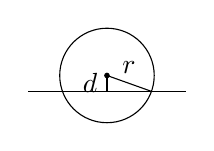
\begin{tikzpicture}[scale=0.4]
\draw (0,0) circle (1.5);
\draw (-2.5,-0.5) -- (2.5,-0.5);
\draw[fill] (0,0) circle (2pt);
\draw (0,0) -- (1.4,-0.5) node[midway,above] {$r$};
\draw (0,0) -- (0,-0.5) node[midway,left] {$d$};
\end{tikzpicture}
&
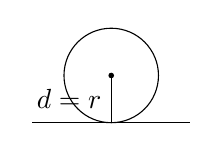
\begin{tikzpicture}[scale=0.4]
\draw (0,0) circle (1.5);
\draw (-2.5,-1.5) -- (2.5,-1.5);
\draw[fill] (0,0) circle (2pt);
\draw (0,0) -- (0,-1.5) node[midway,left] {$d=r$};
\end{tikzpicture}
&
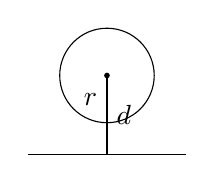
\begin{tikzpicture}[scale=0.4]
\draw (0,0) circle (1.5);
\draw (-2.5,-2.5) -- (2.5,-2.5);
\draw[fill] (0,0) circle (2pt);
\draw (0,0) -- (0,-1.5) node[midway,left] {$r$};
\draw (0,0) -- (0,-2.5) node[midway,right] {$d$};
\end{tikzpicture}
\\
\hline
公共点个数 & 2 & 1 & 0 \\
\hline
判定方法 &
$\begin{aligned}
\Delta &> 0 \quad (\text{代数法}) \\
d &< r \quad (\text{几何法})
\end{aligned}$
&
$\begin{aligned}
\Delta &= 0 \quad (\text{代数法}) \\
d &= r \quad (\text{几何法})
\end{aligned}$
&
$\begin{aligned}
\Delta &< 0 \quad (\text{代数法}) \\
d &> r \quad (\text{几何法})
\end{aligned}$
\\
\hline
\end{tabular}
\end{center}
\vspace{1\baselineskip}

\textcolor{blue}{知识点5.}圆与圆位置关系及公切线

   \begin{center}

\includegraphics[width=10cm]{2.png}
\end{center}

 \begin{center}

\includegraphics[width=10cm]{3.png}
\end{center}
\vspace{1\baselineskip}


\textcolor{blue}{知识点6.}圆系方程

具有某些共同性质的圆的集合称为圆系，它们的方程叫做圆系方程。常见的圆系方程有以下几种：

\begin{enumerate}
    \item \textbf{同心圆系方程}：
    \[
    (x - a)^2 + (y - b)^2 = r^2 \quad (r > 0)
    \]
    其中圆心 \((a,b)\) 为定值，半径 \(r\) 为参数。

    \item \textbf{半径相等的圆系方程}：
    \[
    (x - a)^2 + (y - b)^2 = r^2 \quad (r > 0)
    \]
    其中半径 \(r\) 为定值，圆心 \((a,b)\) 为参数。

    \item \textbf{过直线 \(Ax + By + C = 0\) 与圆 \(x^2 + y^2 + Dx + Ey + F = 0\) 的交点的圆系方程}：
    \[
    x^2 + y^2 + Dx + Ey + F + \lambda(Ax + By + C) = 0 \quad (\lambda \in \mathbf{R})
    \]

    \item \textbf{过两圆 \(C_1: x^2 + y^2 + D_1x + E_1y + F_1 = 0\) 与 \(C_2: x^2 + y^2 + D_2x + E_2y + F_2 = 0\) 的交点的圆系方程}：
    \[
    x^2 + y^2 + D_1x + E_1y + F_1 + \lambda(x^2 + y^2 + D_2x + E_2y + F_2) = 0 \quad (\lambda \neq -1)
    \]
    （其中不含有圆 \(C_2\)，因此注意检验圆 \(C_2\) 是否满足题意，以防产生漏解）。当 \(\lambda = -1\) 时，方程变为
\[
(D_1 - D_2)x + (E_1 - E_2)y + F_1 - F_2 = 0,
\]
表示过两圆交点的直线：
\begin{itemize}
    \item 当两圆是同心圆时，此直线不存在；
    \item 当两圆相交时，此直线为公共弦所在直线；
    \item 当两圆相切时，此直线为两圆的公切线。
\end{itemize}
\end{enumerate}
\vspace{1\baselineskip}


\textcolor{blue}{知识点7.}求解圆的切线

\subsubsection*{求过圆上一点 $(x_0, y_0)$ 的圆的切线方程的两种方法:}

\begin{enumerate}
    \item \textbf{方法一}：
    若 $k \neq 0$ 且 $k$ 存在，先求切点与圆心的连线所在直线的斜率 $k$，再由垂直关系知切线的斜率为 $-\frac{1}{k}$，由点斜式方程可得切线方程；若 $k = 0$ 或 $k$ 不存在，则切线的斜率不存在或为 $0$，从而可直接得切线方程为 $x = x_0$ 或 $y = y_0$。

    \item \textbf{方法二}：利用下列结论解题：
    \begin{enumerate}
        \item 经过圆 $x^2 + y^2 = r^2$ 上一点 $P(x_0, y_0)$ 的切线方程为 $x_0x + y_0y = r^2$。
        \item 经过圆 $(x - a)^2 + (y - b)^2 = r^2$ 上一点 $P(x_0, y_0)$ 的切线方程为 $(x_0 - a)(x - a) + (y_0 - b)(y - b) = r^2$。
        \item 经过圆 $x^2 + y^2 + Dx + Ey + F = 0$ 上一点 $P(x_0, y_0)$ 的切线方程为
        \[
        x_0x + y_0y + D \cdot \frac{x + x_0}{2} + E \cdot \frac{y + y_0}{2} + F = 0.
        \]
    \end{enumerate}
\end{enumerate}

\subsubsection*{求过圆外一点 $(x_0, y_0)$ 的圆的切线方程的方法:}

\begin{enumerate}
    \item \textbf{几何法}：
    设切线方程为 $y - y_0 = k(x - x_0)$，即 $kx - y - kx_0 + y_0 = 0$，由圆心到直线的距离等于半径，可求得 $k$，切线方程即可求出。

    \item \textbf{代数法}：
    设切线方程为 $y - y_0 = k(x - x_0)$，即 $y = kx - kx_0 + y_0$，代入圆的方程，得到一个关于 $x$ 的一元二次方程，由 $\Delta = 0$，求得 $k$，切线方程即可求出。

    \textit{注意}：解题时勿忘考虑斜率不存在的情形。
\end{enumerate}

\begin{tcolorbox}[colback=blue!10,colframe=blue!70!black,title=复习：垂径定理]
\textbf{1. 核心内容}：垂直于弦的直径平分弦，并且平分弦所对的两条弧。

\medskip
\textbf{2. 数学表达式（几何语言）}：
设圆$O$的直径为$AB$，弦为$CD$，且$AB \perp CD$于点$E$，则：
\begin{itemize}
    \item 平分弦：$CE = DE$；
    \item 平分劣弧：$\overset{\frown}{AC} = \overset{\frown}{AD}$；
    \item 平分优弧：$\overset{\frown}{BC} = \overset{\frown}{BD}$。
\end{itemize}

\medskip
\textbf{3. 重要推论}：
平分弦（不是直径）的直径垂直于弦，并且平分弦所对的两条弧。

\medskip
\textbf{4. 拓展结论}：
垂径定理的逆用同样成立，即：
\begin{itemize}
    \item 若直径平分弦（非直径），则直径垂直于弦；
    \item 若直径平分弧，则直径垂直平分弧所对的弦。
\end{itemize}
\end{tcolorbox}
\vspace{1\baselineskip}


\begin{center}
    \subsection*{小节练习}
\end{center}

\noindent\textbf{例一： }已知 \(P_1(4,9)\)，\(P_2(6,3)\) 两点，求以线段 \(P_1P_2\) 为直径的圆的标准方程，并判断点 \(M(6,9)\)，\(N(3,3)\)，\(Q(5,3)\) 在圆上、圆内，还是在圆外
\vspace{3\baselineskip}

\noindent\textbf{例二： }方程 \(x^2 + y^2 + ax + 2ay + 2a^2 + a - 1 = 0\) 表示圆，则 \(a\) 的取值范围是 

\vspace{0.5em}
\noindent
A. \(a < -2\) \quad
B. \(-\dfrac{2}{3} < a < 0\) \quad
C. \(-2 < a < 0\) \quad
D. \(-2 < a < \dfrac{2}{3}\)
\vspace{2\baselineskip}

\noindent\textbf{例三： } 求圆心在直线 \(x - 2y - 3 = 0\) 上，且过点 \(A(2,-3)\)，\(B(-2,-5)\) 的圆的方程
\vspace{3\baselineskip}

\noindent
\textbf{例四: } 设点 \(P(x,y)\) 是圆 \(x^2 + (y+4)^2 = 4\) 上任意一点，则 \(\sqrt{(x-1)^2 + (y-1)^2}\) 的最大值为 \underline{\qquad}.
\vspace{2\baselineskip}

\noindent
\textbf{例五： }（2018天津）在平面直角坐标系中，经过三点 \((0,0)\)，\((1,1)\)，\((2,0)\) 的圆的方程为 \underline{\qquad\qquad\qquad}.
\vspace{2\baselineskip}

\noindent
\textbf{例六： }（2020全国二卷）若过点 \((2,1)\) 的圆与两坐标轴都相切，则圆心到直线 \(2x - y - 3 = 0\) 的距离为 \underline{\qquad}.
\vspace{2\baselineskip}

\noindent\textbf{例七： }求圆心在直线 \(x - y - 4 = 0\) 上，并且经过圆 \(x^2 + y^2 + 6x - 4 = 0\) 与圆 \(x^2 + y^2 + 6y - 28 = 0\) 的交点的圆的方程
\vspace{2\baselineskip}

\noindent\textbf{例八： }(2020河北二模) 圆心在直线 \(3x - y = 0\) 上，与 \(x\) 轴相切，且被直线 \(x - y = 0\) 截得的弦长为 \(2\sqrt{7}\) 的圆的方程为 \underline{\qquad\qquad\qquad}.
\vspace{2\baselineskip}

\noindent\textbf{例九： }(2020·南开二模) 过点 \(P(-\sqrt{3},1)\) 的直线 \(l\) 与圆 \(x^2 + y^2 = 4\) 相切，则直线 \(l\) 在 \(y\) 轴上的截距为 \underline{\qquad}.
\vspace{2\baselineskip}

\noindent\textbf{例十： }（2021实验中学模拟）已知圆 \(C\) 的圆心与点 \((-2,1)\) 关于直线 \(y = x + 1\) 对称，直线 \(3x + 4y - 11 = 0\) 与圆 \(C\) 相交于 \(A,B\) 两点，且 \(|AB| = 6\)，则圆 \(C\) 的方程为 \underline{\qquad\qquad\qquad}.
\vspace{2\baselineskip}

\noindent
\textbf{例十一： }（2021北京）已知圆 \(C: x^2 + y^2 = 4\)，直线 \(l: y = kx + m\)，当 \(k\) 的值发生变化时，直线 \(l\) 被圆 \(C\) 所截得的弦长的最小值为 2，则 \(m\) 的值为 

\vspace{0.5em}
\noindent
A. \(\pm 2\) \quad
B. \(\pm \sqrt{2}\) \quad
C. \(\pm \sqrt{3}\) \quad
D. \(\pm 3\)
\vspace{2\baselineskip}

\noindent
\textbf{例十二： }（多选题）（2021新高考全国一卷）已知点 \(P\) 在圆 \((x-5)^2 + (y-5)^2 = 16\) 上，点 \(A(4,0)\)，\(B(0,2)\)，则

\vspace{0.5em}
\noindent
A. 点 \(P\) 到直线 \(AB\) 的距离小于 10 \\
B. 点 \(P\) 到直线 \(AB\) 的距离大于 2 \\
C. 当 \(\angle PBA\) 最小时，\(|PB| = 3\sqrt{2}\) \\
D. 当 \(\angle PBA\) 最大时，\(|PB| = 3\sqrt{2}\)
\vspace{2\baselineskip}

\noindent
\textbf{例十三： }(2020·浙江) 已知直线 \(y = kx + b\ (k > 0)\) 与圆 \(x^2 + y^2 = 1\) 和圆 \((x - 4)^2 + y^2 = 1\) 均相切，则 \(k = \underline{\qquad}\)，\(b = \underline{\qquad}\).
\vspace{2\baselineskip}

\noindent
\textbf{例十四： }已知 \(A(-2,-2)\)，\(B(-2,6)\)，\(C(4,-2)\) 三点，点 \(P\) 在圆 \(x^2 + y^2 = 4\) 上运动，求 \(|PA|^2 + |PB|^2 + |PC|^2\) 的最大值和最小值。
\vspace{5\baselineskip}
\newpage

\subsection{椭圆}

\textcolor{blue}{知识点1.}椭圆的定义及标准方程
\vspace{1\baselineskip}

把平面内与两个定点 $F_1, F_2$ 的距离的和等于常数（大于 $|F_1F_2|$）的点的轨迹叫做椭圆。这两个定点叫做椭圆的焦点，两焦点间的距离叫做椭圆的焦距，焦距的一半称为半焦距。

椭圆定义用集合表示为：椭圆可看作点集
\[
P = \{ M \mid |MF_1| + |MF_2| = 2a,\ 2a > |F_1F_2| > 0 \}.
\]

\begin{table}[h]
  \centering
  \begin{tabular}{|>{\centering\arraybackslash}m{5cm}|>{\centering\arraybackslash}m{4cm}|>{\centering\arraybackslash}m{3cm}|}
    \hline
    \textbf{标准方程} & \textbf{焦点} & \textbf{焦距} \\
    \hline
    $\dfrac{x^2}{a^2} + \dfrac{y^2}{b^2} = 1\ (a > b > 0)$ & $F_1(-c,0),\ F_2(c,0)$ & \multirow{2}{*}{$2c$, 且 $c^2 = a^2 - b^2$} \\
    \cline{1-2}
    $\dfrac{y^2}{a^2} + \dfrac{x^2}{b^2} = 1\ (a > b > 0)$ & $F_1(0,-c),\ F_2(0,c)$ & \\
    \hline
  \end{tabular}
\end{table}
两种椭圆标准方程的比较:

\begin{table}[h]
  \centering
  \begin{tabular}{|>{\centering\arraybackslash}m{2cm}|>{\centering\arraybackslash}m{3cm}|>{\centering\arraybackslash}m{5cm}|}
    \hline
     & \textbf{相同点} & \textbf{不同点} \\
    \hline
    焦点在 $x$ 轴 & \multirow{2}{*}{\makecell{形状、大小相同，\\$a > b > 0$，\\$b^2 = a^2 - c^2$，\\焦距为 $2c$}} & 方程 $\dfrac{x^2}{a^2} + \dfrac{y^2}{b^2} = 1$ 中，$x^2$对应的分母大\\
    \cline{1-1}\cline{3-3}
    焦点在 $y$ 轴 &  & 方程 $\dfrac{y^2}{a^2} + \dfrac{x^2}{b^2} = 1$ 中，$y^2$对应的分母大\\
    \hline
  \end{tabular}
\end{table}
\vspace{1\baselineskip}

\textcolor{blue}{知识点2.}椭圆标准方程中参数 \(a,b\) 的几何意义:
\vspace{1\baselineskip}

标准方程中的两个参数 \(a,b\) 确定了椭圆的形状和大小，这是椭圆定形的条件。\(a,b,c\) 三个量满足
\[
a^2 = b^2 + c^2,
\]
恰好是一个直角三角形的三条边长，我们把如图所示的直角三角形 \(F_2OM\) 称为椭圆的“特征三角形”。椭圆的特征三角形清晰地反映了参数 \(a,b,c\) 的几何意义。

% 调整图形大小适配盒子，居中显示
\centering
\begin{tikzpicture}[>=Stealth,scale=1.2]
  % 坐标轴
  \draw[->] (-3,0) -- (3,0) node[right] {$x$};
  \draw[->] (0,-2) -- (0,2) node[above] {$y$};
  \fill (0,0) circle (1pt) node[below left] {$O$};
  % 焦点
  \fill (-1,0) circle (1pt) node[below] {$F_1$};
  \fill (1,0) circle (1pt) node[below] {$F_2$};
  % 椭圆
  \draw (0,0) ellipse (2 and 1);
  % 上顶点 M
  \fill (0,1) circle (1pt) node[above right] {$M$};
  % 特征三角形 F2OM（标注边长）
  \draw (1,0) -- (0,1) node[midway,above right] {$a$};
  \draw (0,0) -- (0,1) node[midway,left] {$b$};
  \draw (0,0) -- (1,0) node[midway,below] {$c$};
\end{tikzpicture}

\begin{tcolorbox}[colback=blue!10,colframe=blue!70!black,title=椭圆的一般方程]

\begin{enumerate}
    \item 椭圆标准方程的两种形式可以写成统一的形式：
    \[
    mx^2 + ny^2 = 1 \quad (m > 0,\,n > 0,\,m \neq n).
    \]
    \item 反之，方程 \(Ax^2 + By^2 = C\) 表示椭圆的充要条件是：
    \[
    A,B,C \neq 0,\ \text{且 } A,B,C \text{ 同号},\ A \neq B.
    \]
    \item 特别地：
    \begin{enumerate}
        \item 当 \(0 < B < A\) 或 \(A < B < 0\) 时，方程表示的椭圆的焦点在 \(y\) 轴上；
        \item 当 \(0 < A < B\) 或 \(B < A < 0\) 时，方程表示的椭圆的焦点在 \(x\) 轴上；
        \item 当 \(A = B\) 时，方程表示圆。
    \end{enumerate}
\end{enumerate}
\end{tcolorbox}
\par          % 结束上一段落
\centering    % 切换到居中模式（这是为了重置）
\raggedright  % 再切换回左对齐模式
\vspace{2\baselineskip} 

\;\;\;\;\textcolor{blue}{知识点3.}点与椭圆的位置关系
\vspace{1\baselineskip}

\begin{enumerate}
    \item 根据椭圆的定义判断点 \( P(x_0, y_0) \) 与椭圆的位置关系，有如下结论：
        \[
        \begin{aligned}
        |PF_1| + |PF_2| < 2a &\iff \text{点 } P \text{ 在椭圆内部}; \\
        |PF_1| + |PF_2| = 2a &\iff \text{点 } P \text{ 在椭圆上}; \\
        |PF_1| + |PF_2| > 2a &\iff \text{点 } P \text{ 在椭圆外部}.
        \end{aligned}
        \]
    \item 对于点 \( P(x_0, y_0) \) 与椭圆的位置关系，有如下结论：
        \[
        \begin{aligned}
        \text{点 } P(x_0, y_0) \text{ 在椭圆外} &\iff \frac{x_0^2}{a^2} + \frac{y_0^2}{b^2} > 1; \\
        \text{点 } P(x_0, y_0) \text{ 在椭圆内} &\iff \frac{x_0^2}{a^2} + \frac{y_0^2}{b^2} < 1; \\
        \text{点 } P(x_0, y_0) \text{ 在椭圆上} &\iff \frac{x_0^2}{a^2} + \frac{y_0^2}{b^2} = 1.
        \end{aligned}
        \]
\end{enumerate}
\vspace{1\baselineskip}

\;\;\;\;\textcolor{blue}{知识点4.}椭圆的离心率与基本几何性质
\vspace{1\baselineskip}

\begin{table}[htbp]
    \centering
    \begin{tabular}{|c|c|c|}
        \hline
        \textbf{标准方程} & 
        $\dfrac{x^2}{a^2} + \dfrac{y^2}{b^2} = 1 \ (a > b > 0)$ & 
        $\dfrac{y^2}{a^2} + \dfrac{x^2}{b^2} = 1 \ (a > b > 0)$ \\
        \hline
        \textbf{焦点位置} & 焦点在 $x$ 轴上 & 焦点在 $y$ 轴上 \\
        \hline
        \textbf{图形} & 
        % 焦点在x轴的椭圆（简化实线版）
        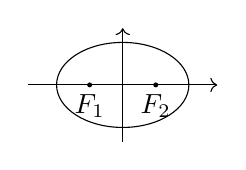
\begin{tikzpicture}[scale=0.6]
            \draw (0,0) ellipse (1.4 and 0.9); % 椭圆实线
            \draw[->] (-2, 0) -- (2, 0); % x轴
            \draw[->] (0, -1.2) -- (0, 1.2); % y轴
            \fill (0,0) circle (0.5pt); % 原点
            \fill (0.7,0) circle (1.5pt) node[below] {$F_2$}; % 焦点
            \fill (-0.7,0) circle (1.5pt) node[below] {$F_1$};
        \end{tikzpicture} & 
        % 焦点在y轴的椭圆（简化实线版）
        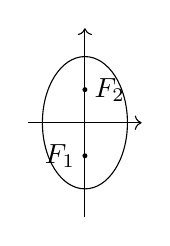
\begin{tikzpicture}[scale=0.6]
            \draw (0,0) ellipse (0.9 and 1.4); % 椭圆实线
            \draw[->] (-1.2, 0) -- (1.2, 0); % x轴
            \draw[->] (0, -2) -- (0, 2); % y轴
            \fill (0,0) circle (0.5pt); % 原点
            \fill (0,0.7) circle (1.5pt) node[right] {$F_2$}; % 焦点
            \fill (0,-0.7) circle (1.5pt) node[left] {$F_1$};
        \end{tikzpicture} \\
        \hline
        \textbf{范围} & 
        $\begin{aligned} -a \le x \le a, \\ -b \le y \le b \end{aligned}$ & 
        $\begin{aligned} -a \le y \le a, \\ -b \le x \le b \end{aligned}$ \\
        \hline
        \textbf{对称性} & 关于 $x$ 轴、$y$ 轴对称，关于原点对称 & 关于 $x$ 轴、$y$ 轴对称，关于原点对称 \\
        \hline
        \textbf{顶点} & 
        $A_1(-a,0), A_2(a,0), B_1(0,-b), B_2(0,b)$ & 
        $A_1(0,-a), A_2(0,a), B_1(-b,0), B_2(b,0)$ \\
        \hline
        \textbf{轴长} & \multicolumn{2}{c|}{长轴长 $|A_1A_2|=2a$，短轴长 $|B_1B_2|=2b$} \\
        \hline
        \textbf{焦距} & \multicolumn{2}{c|}{$|F_1F_2|=2c$} \\
        \hline
        \textbf{离心率} & \multicolumn{2}{c|}{$e = \dfrac{c}{a} \ (0 < e < 1)$} \\
        \hline
    \end{tabular}
\end{table}
\vspace{1\baselineskip}

 对椭圆几何性质的挖掘：

\begin{enumerate}
    \item 椭圆上到中心距离最小的点是短轴的两个端点（即椭圆上的点到椭圆中心的距离的最小值为短半轴长 \(b\)），到中心距离最大的点是长轴的两个端点（即椭圆上的点到椭圆中心的距离的最大值是长半轴长 \(a\)）。
    \item 椭圆上到焦点距离最大的点（称为“远日点”）和最小的点（称为“近日点”）是长轴的两个端点，最大距离为 \(a + c\)，最小距离为 \(a - c\)。
    \item 椭圆的通径：过椭圆的焦点且垂直于长轴的弦叫做椭圆的通径，通径长等于 \(\dfrac{2b^2}{a}\)。
\end{enumerate}


\begin{tcolorbox}[colback=blue!10,colframe=blue!70!black,title=椭圆的范围及参数方程]
\begin{enumerate}
    \item 椭圆是有界的封闭曲线，从椭圆的方程或图形中可以直接看出它的范围。
    \item 观察 \(x,y\) 的取值范围，仿照圆的参数方程可推测出椭圆的参数方程形式：若点 \(M\) 是椭圆 \(\dfrac{x^2}{a^2} + \dfrac{y^2}{b^2} = 1\ (a > b > 0)\) 上的任一点，则可设点 \(M\) 的坐标为 \((a\cos\theta, b\sin\theta)\)（其中 \(\theta \in [0, 2\pi)\)）。这一设法常用于求解涉及椭圆上点的坐标的最值问题。
\end{enumerate}
\end{tcolorbox}

\vspace{1em}

\begin{tcolorbox}[colback=blue!10,colframe=blue!70!black,title=深度剖析椭圆离心率的范围、几何意义及其他表示方式]
\begin{enumerate}
    \item 椭圆离心率 \(e\) 的取值范围：\(e \in (0,1)\)。
    \item \(e\)、\(\dfrac{c}{a}\) 和 \(\dfrac{b}{a}\) 之间可以相互转化，因为由
    \[
    e = \frac{c}{a} = \sqrt{1 - \frac{b^2}{a^2}}
    \]
    可推出 \(\dfrac{b}{a} = \sqrt{1 - e^2}\)。由 \(\dfrac{b}{a} = \sqrt{1 - e^2}\) 可知，当 \(e\) 越趋近于 \(1\) 时，\(\dfrac{b}{a}\) 越趋近于 \(0\)，此时椭圆越扁平；当 \(e\) 越趋近于 \(0\) 时，\(\dfrac{b}{a}\) 越趋近于 \(1\)，此时，椭圆越接近于圆。因此，椭圆的离心率刻画了椭圆的“扁平程度”，离心率 \(e\) 越大，椭圆越扁平，离心率 \(e\) 越小，椭圆越接近于圆。当且仅当 \(a = b, c = 0\) 时，两个焦点重合，椭圆就变为圆，它的方程为 \(x^2 + y^2 = a^2\)。
    \item 如图 3.1.2-1 所示，在 \(\text{Rt}\triangle OBF_1\) 中，\(|BF_1| = a\)，\(|F_1O| = c\)，令 \(\angle F_1BO = \theta\)，则 \(e = \dfrac{c}{a} = \sin\theta\)；在 \(\triangle MF_1F_2\) 中，
    \[
    e = \frac{2c}{2a} = \frac{|F_1F_2|}{|MF_1| + |MF_2|}.
    \]
    \begin{center}
    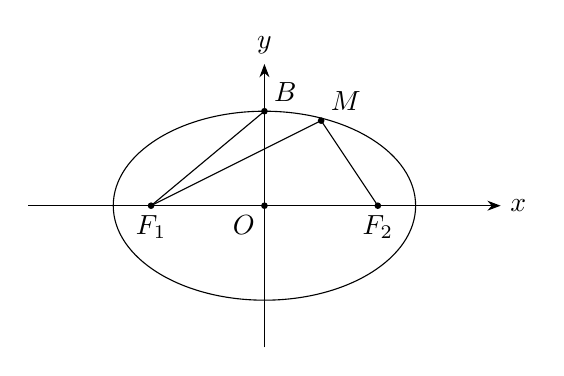
\begin{tikzpicture}[>=Stealth,scale=1.2]
        \draw[->] (-2.5,0) -- (2.5,0) node[right] {$x$};
        \draw[->] (0,-1.5) -- (0,1.5) node[above] {$y$};
        \fill (0,0) circle (1pt) node[below left] {$O$};
        \fill (-1.2,0) circle (1pt) node[below] {$F_1$};
        \fill (1.2,0) circle (1pt) node[below] {$F_2$};
        \fill (0,1) circle (1pt) node[above right] {$B$};
        \fill (0.6,0.9) circle (1pt) node[above right] {$M$};
        \draw (0,0) ellipse (1.6 and 1);
        \draw (-1.2,0) -- (0,1) ;
        \draw (-1.2,0) -- (0.6,0.9) -- (1.2,0);
    \end{tikzpicture}
    \end{center}
\end{enumerate}
\end{tcolorbox}
\vspace{1\baselineskip}

\;\;\;\;\textcolor{blue}{知识点5.}直线与椭圆的位置关系
\vspace{1\baselineskip}

\begin{enumerate}
    \item \textbf{直线与椭圆的三种位置关系}
    类比直线与圆的位置关系，直线与椭圆有相离、相切、相交三种位置关系。
    
    \item \textbf{利用方程讨论直线与椭圆的位置关系}
    设直线方程为 \(y = kx + m\)，椭圆方程为 \(\dfrac{x^2}{a^2} + \dfrac{y^2}{b^2} = 1\ (a > b > 0)\)，联立方程：
    \[
    \begin{cases}
    y = kx + m, \\
    \dfrac{x^2}{a^2} + \dfrac{y^2}{b^2} = 1,
    \end{cases}
    \]
    消去一个变量，得到关于另一个变量的一元二次方程。一般地：
    \[
    \begin{aligned}
    \Delta > 0 &\iff \text{直线与椭圆相交} \iff \text{直线与椭圆有两个公共点}; \\
    \Delta = 0 &\iff \text{直线与椭圆相切} \iff \text{直线与椭圆有且只有一个公共点}; \\
    \Delta < 0 &\iff \text{直线与椭圆相离} \iff \text{直线与椭圆无公共点}.
    \end{aligned}
    \]
    
    \item \textbf{弦长问题}
    设直线 \(l: y = kx + m\) 交椭圆 \(\dfrac{x^2}{a^2} + \dfrac{y^2}{b^2} = 1\ (a > b > 0)\) 于点 \(P_1(x_1, y_1)\)，\(P_2(x_2, y_2)\) 两点，则
    \[
    \begin{aligned}
    |P_1P_2| &= \sqrt{(x_1 - x_2)^2 + (y_1 - y_2)^2} \\
    &= \sqrt{(x_1 - x_2)^2\left[1 + \left(\frac{y_1 - y_2}{x_1 - x_2}\right)^2\right]} = \sqrt{(x_1 - x_2)^2(1 + k^2)} \\
    &= |x_1 - x_2| \cdot \sqrt{1 + k^2}.
    \end{aligned}
    \]
    同理可得 \(|P_1P_2| = |y_1 - y_2| \cdot \sqrt{1 + \frac{1}{k^2}}\ (k \neq 0)\)。
    
    由一元二次方程 \(ax^2 + bx + c = 0\) 或 \(ay^2 + by + c = 0\) 求 \(|x_1 - x_2|\)，\(|y_1 - y_2|\) 的方法有两种：
    \begin{enumerate}
        \item 利用根与系数的关系求解：
        \[
        |x_1 - x_2| = \sqrt{(x_1 + x_2)^2 - 4x_1x_2},\quad |y_1 - y_2| = \sqrt{(y_1 + y_2)^2 - 4y_1y_2};
        \]
        \item 利用求根公式求解：
        \[
        |x_1 - x_2| = \frac{\sqrt{b^2 - 4ac}}{|a|},\quad |y_1 - y_2| = \frac{\sqrt{b^2 - 4ac}}{|a|}.
        \]
    \end{enumerate}
\end{enumerate}
\vspace{1\baselineskip}

\;\;\;\;\textcolor{blue}{知识点6.}椭圆的第二、第三定义
\vspace{1\baselineskip}

\begin{enumerate}
    \item \textbf{椭圆的第二定义}
    \[
    \{ P \mid \frac{|PF|}{d} = e,\ 0 < e < 1 \}
    \]
    其中 \(F\) 为定点，\(l\) 为定直线，\(e\) 为离心率，\(F \notin l\)，\(d\) 表示点 \(P\) 到直线 \(l\) 的距离。

    \item \textbf{椭圆的第三定义}
    \[
    \{ P \mid k_{PA} \cdot k_{PB} = e^2 - 1,\ 0 < e < 1 \}
    \]
    其中 \(k_{PA}, k_{PB}\) 分别表示点 \(P\) 与两定点 \(A, B\) 连线的斜率，\(e\) 为离心率。

    \textbf{注意}：第三定义中的定点在 \(x\) 轴上，且利用该定义得出的轨迹方程不包括这两个定点。


    \item \textbf{由椭圆的第二定义探究椭圆的几何性质}
    \begin{enumerate}
        \item \textbf{准线}
        \begin{itemize}
            \item 椭圆 \(\dfrac{x^2}{a^2} + \dfrac{y^2}{b^2} = 1\ (a > b > 0)\) 的准线方程为：\(x = \pm \dfrac{a^2}{c}\)；
            \item 椭圆 \(\dfrac{y^2}{a^2} + \dfrac{x^2}{b^2} = 1\ (a > b > 0)\) 的准线方程为：\(y = \pm \dfrac{a^2}{c}\)。
        \end{itemize}
        两准线间的距离为 \(\dfrac{2a^2}{c}\)，焦点到相应准线的距离为 \(\dfrac{b^2}{c}\)。

        \item \textbf{焦半径}
        设 \(P(x_1, y_1)\) 为椭圆上任一点：
        \begin{itemize}
            \item 对于 \(\dfrac{x^2}{a^2} + \dfrac{y^2}{b^2} = 1\ (F_1,F_2\) 为左、右焦点\()\)：
            \[
            |PF_1| = a + ex_1, \quad |PF_2| = a - ex_1;
            \]
            \item 对于 \(\dfrac{y^2}{a^2} + \dfrac{x^2}{b^2} = 1\ (F_1,F_2\) 为上、下焦点\()\)：
            \[
            |PF_1| = a - ey_1, \quad |PF_2| = a + ey_1.
            \]
        \end{itemize}
    \end{enumerate}
\end{enumerate}
\vspace{1\baselineskip}

\;\;\;\;\textcolor{blue}{知识点7.}与椭圆焦点三角形有关的常用公式
\vspace{1\baselineskip}

\begin{enumerate}
    \item 焦点三角形的周长 \( L = 2a + 2c \)。
    \item 在焦点三角形 \( MF_1F_2 \) 中，由余弦定理可得
    \[
    |F_1F_2|^2 = |MF_1|^2 + |MF_2|^2 - 2|MF_1||MF_2| \cdot \cos \angle F_1MF_2.
    \]
    \item 设焦点在 \( x \) 轴上的椭圆上任一点 \( M(x_M, y_M) \ (y_M \neq 0) \)，则焦点三角形的面积
    \[
    S_{\triangle F_1MF_2} = c|y_M| = \frac{1}{2}|MF_1||MF_2| \cdot \sin \angle F_1MF_2 = b^2\tan \frac{\angle F_1MF_2}{2}.
    \]
\end{enumerate}

\begin{center}
    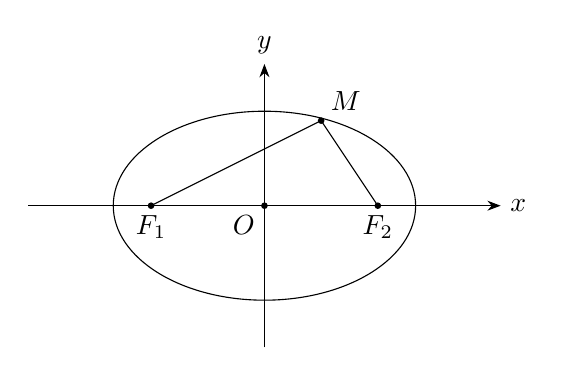
\begin{tikzpicture}[>=Stealth,scale=1.2]
        \draw[->] (-2.5,0) -- (2.5,0) node[right] {$x$};
        \draw[->] (0,-1.5) -- (0,1.5) node[above] {$y$};
        \fill (0,0) circle (1pt) node[below left] {$O$};
        \fill (-1.2,0) circle (1pt) node[below] {$F_1$};
        \fill (1.2,0) circle (1pt) node[below] {$F_2$};
        \fill (0.6,0.9) circle (1pt) node[above right] {$M$};
        \draw (0,0) ellipse (1.6 and 1);
        \draw (-1.2,0) -- (0.6,0.9) -- (1.2,0);
    \end{tikzpicture}
\end{center}

\vspace{1\baselineskip}

\begin{center}
    \subsection*{微专题：椭圆离心率的计算}   
\end{center}
\vspace{1\baselineskip}

\begin{tcolorbox}[colback=blue!10,colframe=blue!70!black,title=求椭圆离心率的基本思路]
\begin{enumerate}
    \item 求椭圆离心率的值，关键是寻找 \(a,b,c\) 所满足的等量关系，这就需要画图分析，充分利用图形的直观性来解决问题，具体解题时还应注意利用“\(b^2 = a^2 - c^2\)”消去 \(b\)，在找到 \(a,b,c\) 的等量关系后需要两边平方，这样才便于消去 \(b\)。
    \item 需要注意的是：我们通过题设条件列出的关于\(a,b,c\) 的等式必须是其次的，这样我们才可以通过同时除以\(c\)的操作来构造出离心率的表达式。
    \item 计算离心率的常见形式：
    \[
    \begin{aligned}
    e &= \frac{c}{a} = \frac{2c}{2a} = \frac{|F_1F_2|}{|PF_1| + |PF_2|} = \frac{\sin \angle F_1PF_2}{\sin \angle PF_1F_2 + \sin \angle PF_2F_1}, \\
    e &= \frac{c}{a} = \sqrt{\frac{a^2 - b^2}{a^2}} = \sqrt{1 - \frac{b^2}{a^2}}.
    \end{aligned}
    \]
\end{enumerate}
\end{tcolorbox}
\vspace{1\baselineskip}

\noindent\subsection*{例题一： }
椭圆 \(\dfrac{x^2}{a^2} + \dfrac{y^2}{b^2} = 1\ (a > b > 0)\) 的一个焦点为 \(F\)，该椭圆上有一点 \(A\)，满足 \(\triangle OAF\) 是等边三角形（\(O\) 为坐标原点），则椭圆的离心率是 \underline{\quad\quad\quad}。

\paragraph{解析:}
设点 \(F(c,0)\)，由 \(\triangle OAF\) 是等边三角形，得 \(A\left(\dfrac{c}{2},\dfrac{\sqrt{3}c}{2}\right)\)。
因为点 \(A\) 在椭圆上，所以
\[
\frac{c^2}{4a^2} + \frac{3c^2}{4b^2} = 1 \quad \text{①}
\]
在椭圆中有 \(a^2 = b^2 + c^2\) ②，联立①②，得 \(c^2 = (4 - 2\sqrt{3})a^2\)，即 \(c = (\sqrt{3} - 1)a\)，则其离心率
\[
e = \frac{c}{a} = \sqrt{3} - 1.
\]

\vspace{1em}

\subsection*{例题二： }
椭圆 \(\dfrac{x^2}{a^2} + \dfrac{y^2}{b^2} = 1\ (a > b > 0)\) 的两焦点为 \(F_1,F_2\)，以 \(F_1F_2\) 为边作正三角形，若椭圆恰好平分正三角形的另两条边，则椭圆的离心率为 \underline{\quad\quad\quad}。

\paragraph{解析:}
连接 \(F_1N\)，因为 \(\triangle DF_1F_2\) 为正三角形，\(N\) 为 \(DF_2\) 的中点，所以 \(F_1N \perp F_2N\)。
\paragraph{方法一:}
因为 \(|NF_2| = |OF_2| = c\)，所以
\[
|NF_1| = \sqrt{|F_1F_2|^2 - |NF_2|^2} = \sqrt{4c^2 - c^2} = \sqrt{3}c,
\]
由椭圆的定义可知 \(|NF_1| + |NF_2| = 2a\)，所以
\[
\sqrt{3}c + c = 2a \implies a = \frac{(\sqrt{3} + 1)c}{2},
\]
故
\[
e = \frac{c}{a} = \frac{2}{\sqrt{3} + 1} = \sqrt{3} - 1.
\]

\paragraph{方法二:}
注意到在焦点三角形 \(NF_1F_2\) 中，\(\angle NF_1F_2 = 30^\circ\)，\(\angle NF_2F_1 = 60^\circ\)，\(\angle F_1NF_2 = 90^\circ\)，则由正弦定理可得
\[
\frac{2c}{\sin \angle F_1NF_2} = \frac{|F_1N|}{\sin \angle F_1F_2N} = \frac{|F_2N|}{\sin \angle NF_1F_2},
\]
即
\[
\frac{2c}{\sin 90^\circ} = \frac{|F_1N|}{\sin 60^\circ} = \frac{|F_2N|}{\sin 30^\circ},
\]
所以
\[
\frac{2c}{\sin 90^\circ} = \frac{|F_1N| + |F_2N|}{\sin 30^\circ + \sin 60^\circ} = \frac{2a}{\sin 30^\circ + \sin 60^\circ},
\]
故
\[
e = \frac{c}{a} = \frac{\sin 90^\circ}{\sin 30^\circ + \sin 60^\circ} = \frac{1}{\frac{1}{2} + \frac{\sqrt{3}}{2}} = \sqrt{3} - 1.
\]


\vspace{1em}

\subsection*{例题三（2021浙江）}
已知椭圆 \(\dfrac{x^2}{a^2} + \dfrac{y^2}{b^2} = 1\ (a > b > 0)\)，焦点 \(F_1(-c,0)\)，\(F_2(c,0)\ (c > 0)\)。若过 \(F_1\) 的直线和圆 \(\left(x - \dfrac{1}{2}c\right)^2 + y^2 = c^2\) 相切，与椭圆在第一象限交于点 \(P\)，且 \(PF_2 \perp x\) 轴，则该直线的斜率是 \underline{\quad\quad\quad}，椭圆的离心率是 \underline{\quad\quad\quad}。

\paragraph{解析:}
设过 \(F_1\) 的直线与圆的切点为 \(M\)，圆心 \(A\left(\dfrac{1}{2}c,0\right)\)，则 \(|AM| = c\)，\(|AF_1| = \dfrac{3}{2}c\)，所以
\[
|MF_1| = \frac{\sqrt{5}}{2}c,
\]
所以该直线的斜率
\[
k = \frac{|AM|}{|MF_1|} = \frac{c}{\frac{\sqrt{5}}{2}c} = \frac{2\sqrt{5}}{5}.
\]

因为 \(PF_2 \perp x\) 轴，所以 \(|PF_2| = \dfrac{b^2}{a}\)，又 \(|F_1F_2| = 2c\)，所以
\[
k = \frac{2\sqrt{5}}{5} = \frac{\dfrac{b^2}{a}}{2c} = \frac{a^2 - c^2}{2ac} = \frac{1 - e^2}{2e},
\]
得
\[
e = \frac{\sqrt{5}}{5}.
\]

\begin{center}
    \subsection*{小节练习}
\end{center}
\vspace{1\baselineskip}

% ========== 选择题部分 ==========
% 例一
\noindent\textbf{例一： }(2021新高考一卷)已知$F_1,F_2$是椭圆$C:\dfrac{x^2}{9}+\dfrac{y^2}{4}=1$的两个焦点，点$M$在$C$上，则$|MF_1|\cdot|MF_2|$的最大值为
\vspace{0.5em}

\noindent
A. $13$ \quad
B. $12$ \quad
C. $9$ \quad
D. $6$
\vspace{2\baselineskip}

% 例二
\noindent\textbf{例二： }(2019全国一卷)已知椭圆$C$的焦点为$F_1(-1,0)$，$F_2(1,0)$，过$F_2$的直线与$C$交于$A$，$B$两点。若$|AF_2|=2|F_2B|$，$|AB|=|BF_1|$，则$C$的方程为
\vspace{0.5em}

\noindent
A. $\dfrac{x^2}{2}+y^2=1$ \quad
B. $\dfrac{x^2}{3}+\dfrac{y^2}{2}=1$ \quad
C. $\dfrac{x^2}{4}+\dfrac{y^2}{3}=1$ \quad
D. $\dfrac{x^2}{5}+\dfrac{y^2}{4}=1$
\vspace{2\baselineskip}

% 例三
\noindent\textbf{例三： }(2018全国二卷)已知$F_1,F_2$是椭圆$C:\dfrac{x^2}{a^2}+\dfrac{y^2}{b^2}=1\ (a>b>0)$的左、右焦点，$A$是$C$的左顶点，点$P$在过$A$且斜率为$\dfrac{\sqrt{3}}{6}$的直线上，$\triangle PF_1F_2$为等腰三角形，$\angle F_1F_2P=120^\circ$，则$C$的离心率为
\vspace{0.5em}

\noindent
A. $\dfrac{2}{3}$ \quad
B. $\dfrac{1}{2}$ \quad
C. $\dfrac{1}{3}$ \quad
D. $\dfrac{1}{4}$
\vspace{2\baselineskip}

% ========== 填空题部分 ==========
% 例四
\noindent\textbf{例四： }如图3.1-6，设$A$，$B$两点的坐标分别为$(-5,0)$，$(5,0)$。直线$AM$，$BM$相交于点$M$，且它们的斜率之积是$-\dfrac{4}{9}$，求点$M$的轨迹方程\underline{\hspace{8em}}。
\vspace{2\baselineskip}

% 例五
\noindent\textbf{例五： }动点$M(x,y)$与定点$F(4,0)$的距离和$M$到定直线$l:x=\dfrac{25}{4}$的距离的比是常数$\dfrac{4}{5}$，求动点$M$的轨迹\underline{\hspace{8em}}。
\vspace{2\baselineskip}

% 例六
\noindent\textbf{例六： }已知椭圆$\dfrac{x^2}{25}+\dfrac{y^2}{9}=1$，直线$l:4x-5y+40=0$。椭圆上是否存在一点，使得：
\par (1) 它到直线$l$的距离最小？最小距离是多少？
\par (2) 它到直线$l$的距离最大？最大距离是多少？
\vspace{5\baselineskip}

% 例七
\noindent\textbf{例七： }已知椭圆$\dfrac{x^2}{4}+\dfrac{y^2}{9}=1$，一组平行直线的斜率是$\dfrac{3}{2}$。
\par (1) 这组直线何时与椭圆有两个公共点？
\par (2) 当它们与椭圆有两个公共点时，证明这些直线被椭圆截得的线段的中点在同一条直线上。
\vspace{8\baselineskip}

% 例八
\noindent\textbf{例八： }已知椭圆的标准方程为$\dfrac{x^2}{25}+\dfrac{y^2}{m^2}=1\ (m>0)$，并且焦距为6，则实数$m$的值为\underline{\hspace{6em}}。
\vspace{2\baselineskip}

% 例九
\noindent\textbf{例九： }(辽宁高考题)已知椭圆$C:\dfrac{x^2}{9}+\dfrac{y^2}{4}=1$，点$M$与$C$的焦点不重合。若$M$关于$C$的焦点的对称点分别为$A$，$B$，线段$MN$的中点在$C$上，则$|AN|+|BN|=$\underline{\hspace{5em}}。
\vspace{2\baselineskip}

\noindent\textbf{例十： }
\begin{minipage}[t]{0.9\textwidth}
如图，圆$O$的半径为定长$r$，$A$是圆$O$内一个定点，$P$是圆$O$上任意一点。线段$AP$的垂直平分线$l$和半径$OP$相交于点$Q$，当点$P$在圆上运动时，点$Q$的轨迹是什么？为什么？
\end{minipage}
\hfill
\begin{minipage}[t]{0.25\textwidth}
\centering
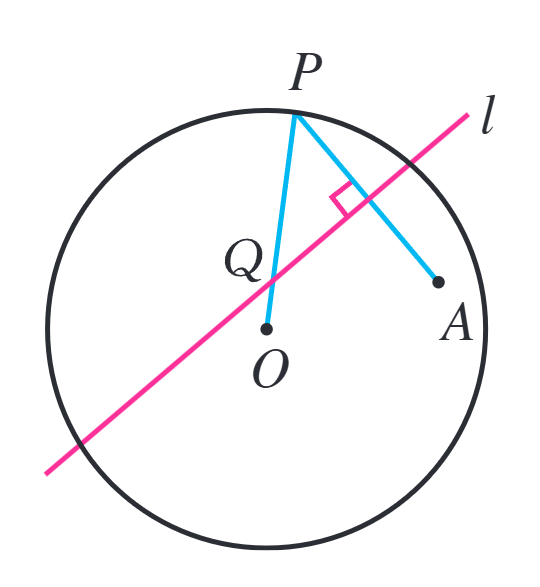
\includegraphics[width=\linewidth]{4.png}
\end{minipage}
\vspace{2\baselineskip}

\subsection{双曲线}
\vspace{2\baselineskip}

\textcolor{blue}{知识点1.}双曲线的定义及标准方程
\vspace{2\baselineskip}

\begin{table}[htbp]
  \centering
  \renewcommand{\arraystretch}{1.8} % 调整行高，避免内容拥挤
  \begin{tabular}{|c|p{13cm}|}
    \hline
    \textbf{定义} & 平面内与两个定点 $F_1,F_2$ 的距离的差的绝对值等于非零常数(小于 $|F_1F_2|$) 的点的轨迹叫做双曲线，分左右两支，常数用 $2a$ 表示。 \\
    \hline
    \textbf{焦点} & 两个定点 $F_1,F_2$ 叫做双曲线的焦点。 \\
    \hline
    \textbf{焦距} & 两焦点间的距离叫做双曲线的焦距，用 $2c(c>0)$ 表示。 \\
    \hline
    \makecell{\textbf{集合}\\\textbf{语言}} & $P = \left\{ M \mid \left|\left|MF_1\right| - \left|MF_2\right|\right| = 2a, 0 < 2a < |F_1F_2| \right\}$。 \\
    \hline
  \end{tabular}
\end{table}

% 两个表格之间的间距
\vspace{1em}

% ========== 第二个表格：双曲线标准方程与性质 ==========
\begin{table}[htbp]
  \centering
  \renewcommand{\arraystretch}{2} % 控制行高，避免内容拥挤
  % 列格式优化：第一列固定宽度+居中，避免文字错位
  \begin{tabular}{|m{2cm}<{\centering}|c|c|}
    \hline
    \textbf{标准方程} & $\dfrac{x^2}{a^2} - \dfrac{y^2}{b^2} = 1 \ (a>0,b>0)$ & $\dfrac{y^2}{a^2} - \dfrac{x^2}{b^2} = 1 \ (a>0,b>0)$ \\
    \hline
    \textbf{图形} & 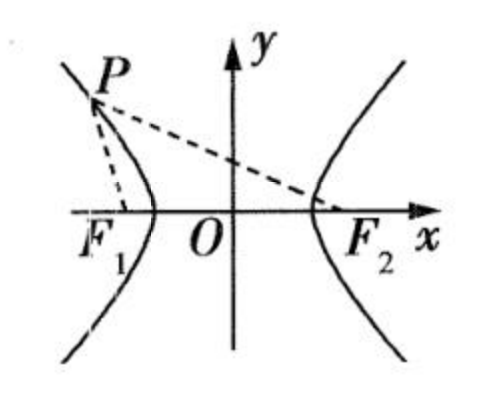
\includegraphics[width=0.3\textwidth]{双曲线x.png} & 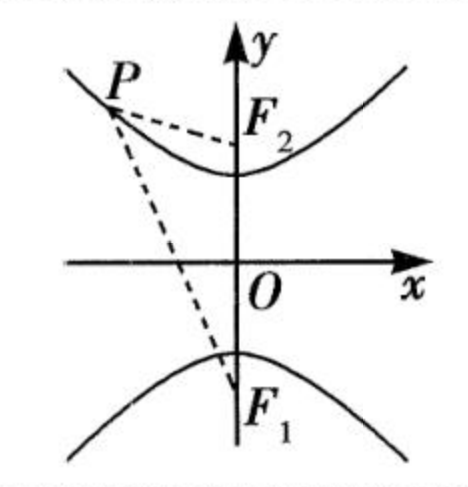
\includegraphics[width=0.3\textwidth]{双曲线y.png} \\
    \hline
    \textbf{焦点位置} & 焦点在 $x$ 轴上 & 焦点在 $y$ 轴上 \\
    \hline
    \textbf{焦点坐标} & $F_1(-c,0),\ F_2(c,0)$ & $F_1(0,-c),\ F_2(0,c)$ \\
    \hline
    \textbf{焦距} & \multicolumn{2}{c|}{$\left|F_1F_2\right| = 2c$} \\
    \hline
    % 核心修正的行，彻底解决报错
    \textbf{异同点} & \multicolumn{2}{p{10cm}|}{
      相同点：大小、形状相同，都有 $a>0,b>0$，$a,b,c$ 的关系都满足 $b^2 = c^2 - a^2$。\par
      不同点：焦点的位置和坐标不同。
    } \\
    \hline
  \end{tabular}
\end{table}

\begin{tcolorbox}[colback=blue!10,colframe=blue!70!black,title=]
方程 $\dfrac{x^2}{m}+\dfrac{y^2}{n}=1$ 既可以表示椭圆又可以表示双曲线。
\begin{enumerate}
    \renewcommand{\labelenumi}{(\arabic{enumi})} % 自定义编号为(1)(2)格式，和原文一致
    \item 当方程表示椭圆时，$m,n$ 应满足 $m>n>0$ 或 $n>m>0$。
    \item 当方程表示双曲线时，$m,n$ 应满足 $mn<0$；当 $m>0,n<0$ 时，方程表示焦点在 $x$ 轴上的双曲线；当 $m<0,n>0$ 时，方程表示焦点在 $y$ 轴上的双曲线。
\end{enumerate}

\noindent 若不确定焦点位置，则可设双曲线的方程为 $\dfrac{x^2}{m}+\dfrac{y^2}{n}=1\ (mn<0)$ 或 $mx^2+ny^2=1\ (mn<0)$。
\end{tcolorbox}
\vspace{2\baselineskip}

\textcolor{blue}{知识点2.}双曲线的焦点三角形
\vspace{2\baselineskip}

如上图，$P$ 是双曲线 $\dfrac{x^2}{a^2}-\dfrac{y^2}{b^2}=1\ (a>0,b>0)$ 上任意一点，$F_1,F_2$ 分别是双曲线的左、右焦点，当点 $P,F_1,F_2$ 不在同一条直线上时，它们构成一个三角形——焦点三角形。


\noindent 设 $\angle F_1PF_2=\theta$，则由双曲线的定义及余弦定理得，

 $$ \left|\left|PF_1\right| - \left|PF_2\right|\right| = 2a \Leftrightarrow \left|PF_1\right|^2 + \left|PF_2\right|^2 - 2\left|PF_1\right|\cdot\left|PF_2\right| = 4a^2 \quad (1), $$

 $$ \left|PF_1\right|^2 + \left|PF_2\right|^2 - 2\left|PF_1\right|\cdot\left|PF_2\right|\cdot\cos\theta = \left|F_1F_2\right|^2 = 4c^2 \quad (2).$$


\noindent 由 $(2) - (1)$ 得：
$$2\left|PF_1\right|\cdot\left|PF_2\right|\cdot(1-\cos\theta) = 4c^2 - 4a^2,$$

\noindent 则 $\boldsymbol{\left|PF_1\right|\cdot\left|PF_2\right| = \dfrac{2b^2}{1-\cos\theta}}$。（只能用于选择、填空题）

\vspace{0.5em}
\noindent 又三角形面积公式：
$$S_{\triangle PF_1F_2} = \dfrac{1}{2}\left|PF_1\right|\cdot\left|PF_2\right|\cdot\sin\theta,$$

\noindent 代入上式可得：
$$\boldsymbol{S_{\triangle PF_1F_2} = b^2\cdot\dfrac{\sin\theta}{1-\cos\theta} = \dfrac{b^2}{\tan\dfrac{\theta}{2}}}$$
（只能用于选择、填空题）





\begin{tcolorbox}[colback=blue!10,colframe=blue!70!black,title=共焦点双曲线方程的设法]
\begin{enumerate}
    \item 与椭圆$\dfrac{x^2}{a^2}+\dfrac{y^2}{b^2}=1\ (a>b>0)$有公共焦点的双曲线方程为$\dfrac{x^2}{a^2+\lambda}+\dfrac{y^2}{b^2+\lambda}=1\ (-a^2<\lambda<-b^2)$；与椭圆$\dfrac{y^2}{a^2}+\dfrac{x^2}{b^2}=1\ (a>b>0)$有公共焦点的双曲线方程为$\dfrac{y^2}{a^2+\lambda}+\dfrac{x^2}{b^2+\lambda}=1\ (-a^2<\lambda<-b^2)$。
    \item 与双曲线$\dfrac{x^2}{a^2}-\dfrac{y^2}{b^2}=1\ (a>0,b>0)$有公共焦点的双曲线方程为$\dfrac{x^2}{a^2+\lambda}-\dfrac{y^2}{b^2-\lambda}=1\ (-a^2<\lambda<b^2)$；与双曲线$\dfrac{y^2}{a^2}-\dfrac{x^2}{b^2}=1\ (a>0,b>0)$有公共焦点的双曲线方程为$\dfrac{y^2}{a^2+\lambda}-\dfrac{x^2}{b^2-\lambda}=1\ (-a^2<\lambda<b^2)$。
\end{enumerate}
\end{tcolorbox}
\vspace{2\baselineskip}

\textcolor{blue}{知识点3.}双曲线的离心率与基本几何性质
\vspace{2\baselineskip}

\begin{table}[H]
  \centering
  \renewcommand{\arraystretch}{2.2} % 调整行高，避免内容拥挤
  % 列格式：第一列固定宽度+居中，后两列居中，完整竖线边框
  \begin{tabular}{|m{2cm}<{\centering}|c|c|}
    \hline
    \textbf{标准方程} & $\dfrac{x^2}{a^2}-\dfrac{y^2}{b^2}=1\ (a>0,b>0)$ & $\dfrac{y^2}{a^2}-\dfrac{x^2}{b^2}=1\ (a>0,b>0)$ \\
    \hline
    \textbf{图形} & 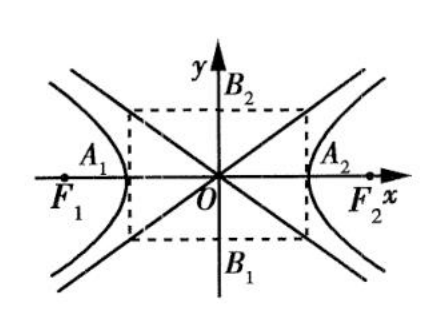
\includegraphics[width=0.35\textwidth]{x.png} & 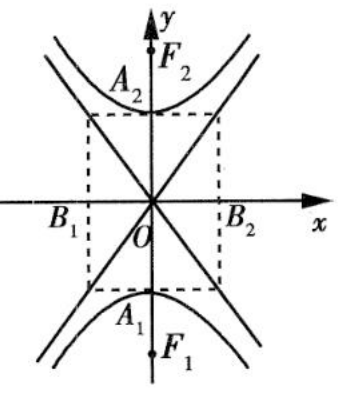
\includegraphics[width=0.25\textwidth]{y.png} \\
    \hline
    \textbf{范围} & $|x| \geqslant a,\ y \in \mathbf{R}$ & $|y| \geqslant a,\ x \in \mathbf{R}$ \\
    \hline
    \textbf{对称性} & \multicolumn{2}{c|}{对称轴：$x$ 轴、$y$ 轴 \quad 对称中心：原点} \\
    \hline
    \textbf{顶点} & $A_1(-a,0),\ A_2(a,0)$ & $A_1(0,-a),\ A_2(0,a)$ \\
    \hline
    \textbf{轴} & \multicolumn{2}{p{11cm}|}{
      线段$A_1A_2$是双曲线的实轴，线段$B_1B_2$是双曲线的虚轴。实轴长$|A_1A_2|=2a$，虚轴长$|B_1B_2|=2b$
    } \\
    \hline
    \textbf{渐近线} & 直线$y = \pm \dfrac{b}{a}x$ & 直线$y = \pm \dfrac{a}{b}x$ \\
    \hline
    \textbf{离心率} & \multicolumn{2}{c|}{$e = \dfrac{c}{a}\ (e>1)$} \\
    \hline
  \end{tabular}
\end{table}
\vspace{2\baselineskip}

\textcolor{blue}{知识点4.}双曲线标准方程中参数$a,b$的几何意义
\vspace{2\baselineskip}

如下图所示的$\triangle MOF_2$也可称为特征三角形。焦点$F_2(c,0)$到渐近线的距离
$$\left|MF_2\right| = \frac{\left|bc \pm a\cdot 0\right|}{\sqrt{a^2+b^2}} = \frac{bc}{c} = b,$$
即双曲线的焦点到渐近线的距离为虚半轴长。而且在$\triangle MOF_2$中，很容易得到
$$\cos\theta = \frac{1}{e}.$$
故若知道两条渐近线的夹角，我们可以很容易求出双曲线的离心率。

% 居中插图
\begin{figure}[htbp]
  \centering
  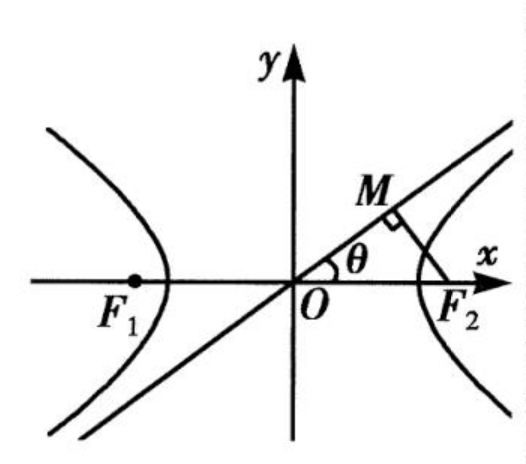
\includegraphics[width=0.5\textwidth]{5.png}
\end{figure}

\noindent 对于椭圆，在特征三角形$B_2OF_2$中（$B_2$为上顶点，$F_2$为右焦点，$O$为原点），记$\theta' = \angle B_2F_2O$，由于$\cos\theta' = e$，所以$e$越大，$\theta'$越小，从而椭圆就越扁，相反就越圆；而对于双曲线，考虑到$e = \dfrac{1}{\cos\theta}$（如图3.2.2-1），则$e$越大，$\theta$越大，即渐近线张口越大，双曲线的开口就越大。
\vspace{2\baselineskip}

\textcolor{blue}{知识点5.}双曲线的第二、第三定义
\vspace{1\baselineskip}

\begin{enumerate}
    \item \textbf{双曲线的第二定义}：$\left\{ P \mid \dfrac{|PF|}{d} = e,\, e>1,\, F \notin l \right\}$，其中$F$为定点，$l$为定直线，$e$为离心率，$d$为点$P$到直线$l$的距离（其中$F$为左焦点时，$l$为左准线$x = -\dfrac{a^2}{c}$；$F$为右焦点时，$l$为右准线$x = \dfrac{a^2}{c}$）。
    \item \textbf{双曲线的第三定义}：$\left\{ P \mid k_{PA} \cdot k_{PB} = e^2 - 1,\, e>1 \right\}$，其中$k_{PA},k_{PB}$分别表示点$P$与两定点$A,B$连线的斜率，$e$为离心率（注意，此时确定的双曲线不包含两个顶点，且焦点在$x$轴上）。
\end{enumerate}

\begin{tcolorbox}[colback=blue!10,colframe=blue!70!black,title=双曲线的通径]
过焦点且与焦点所在的轴垂直的直线被双曲线截得的线段叫做双曲线的通径。

对于双曲线$\dfrac{x^2}{a^2}-\dfrac{y^2}{b^2}=1\ (a>0,b>0)$，将$x=c$代入双曲线的方程可得：
\begin{align*}
\dfrac{y^2}{b^2} &= \dfrac{c^2}{a^2} - 1 \\
&= \dfrac{c^2 - a^2}{a^2} = \dfrac{b^2}{a^2},
\end{align*}
所以直线$x=c$与双曲线的两个交点为$A\left(c,\dfrac{b^2}{a}\right)$、$B\left(c,-\dfrac{b^2}{a}\right)$，计算得通径长$|AB| = \dfrac{2b^2}{a}$。

同理，可求得双曲线$\dfrac{y^2}{a^2}-\dfrac{x^2}{b^2}=1\ (a>0,b>0)$的通径长也是$\dfrac{2b^2}{a}$。
\end{tcolorbox}
\vspace{1\baselineskip}

\textcolor{blue}{知识点6.}直线与双曲线的位置关系
\vspace{1\baselineskip}

\noindent 一般地，设直线方程为 $y = kx + m\ (m \neq 0)$，双曲线方程为 $\dfrac{x^2}{a^2} - \dfrac{y^2}{b^2} = 1\ (a>0,b>0)$，将 $y = kx + m$ 代入 $\dfrac{x^2}{a^2} - \dfrac{y^2}{b^2} = 1$，消去 $y$ 并化简，得
$$(b^2 - a^2k^2)x^2 - 2a^2mkx - a^2m^2 - a^2b^2 = 0.$$

\begin{enumerate}
    % 自定义编号为带圈数字，和原文格式完全一致
    \renewcommand{\labelenumi}{\textcircled{\arabic{enumi}}}
    \item 当 $b^2 - a^2k^2 = 0$，即 $k = \pm \dfrac{b}{a}$ 时，直线与渐近线平行，则直线与双曲线只有一个公共点。
    \item 当 $b^2 - a^2k^2 \neq 0$，即 $k \neq \pm \dfrac{b}{a}$ 时，判别式 $\Delta > 0 \Leftrightarrow$ 直线与双曲线相交，有两个公共点；判别式 $\Delta = 0 \Leftrightarrow$ 直线与双曲线相切，有且只有一个公共点；判别式 $\Delta < 0 \Leftrightarrow$ 直线与双曲线相离，没有公共点。
\end{enumerate}
\vspace{1\baselineskip}

\textcolor{blue}{知识点7.}双曲线与椭圆的异同
\vspace{1\baselineskip}

双曲线和椭圆在表达式、离心率、通经长、准线、对称性方面的异同显而易见，我们下面列举一些对同学们来说相对陌生的异同点
\vspace{1\baselineskip}

\begin{table}[htbp]
  \centering
  \renewcommand{\arraystretch}{2.2} % 调整行高，避免内容拥挤
  % 列格式：固定宽度+居中对齐，和原图边框完全一致
  \begin{tabular}{|m{4cm}<{\centering}|m{5cm}<{\centering}|m{5cm}<{\centering}|}
    \hline
     & \textbf{椭圆} & \textbf{双曲线} \\
    \hline
    \makecell{焦半径 $r_1,r_2$\\与点 $P$ 坐标\\$(x_P,\ y_P)$ 的关系} 
    & \makecell{$r_1 = a + e x_P$\\$r_2 = a - e x_P$} 
    & \makecell{当点 $P$ 在双曲线右支上时：\\$r_1 = e x_P + a$，$r_2 = e x_P - a$\\当点 $P$ 在双曲线左支上时：\\$r_1 = -e x_P - a$，$r_2 = -e x_P + a$} \\
    \hline
    \makecell{$\angle F_2PF_1 = \theta$\\$\angle PF_1F_2 = \alpha$\\$\angle PF_2F_1 = \beta$} 
    & \makecell{$1 + \cos\theta = \dfrac{2b^2}{r_1r_2}$\\$S_{\triangle PF_1F_2} = b^2\tan\dfrac{\theta}{2} = c|y_P|$} 
    & \makecell{$1 - \cos\theta = \dfrac{2b^2}{r_1r_2}$\\$S_{\triangle PF_1F_2} = b^2\cot\dfrac{\theta}{2} = c|y_P|$} \\
    \hline
    \makecell{离心率与 $\alpha,\beta$\\的关系} 
    & $e = \dfrac{\sin(\alpha+\beta)}{\sin\alpha + \sin\beta}$ 
    & $e = \dfrac{\sin(\alpha+\beta)}{\left|\sin\alpha - \sin\beta\right|}$ \\
    \hline
  \end{tabular}
\end{table}
\newpage

\begin{tcolorbox}[colback=blue!10,colframe=blue!70!black,title=圆锥曲线的参数方程焦半径公式]
\begin{enumerate}
    \item \textbf{椭圆}：
    参数方程为 $\begin{cases} x = a\cos\varphi \\ y = b\sin\varphi \end{cases}$（$\varphi$ 为离心角），
    焦半径公式为：
    \begin{align*}   
    |MF_1| &= \frac{b^2}{a-c \cos \alpha }, \\
    |MF_2| &= \frac{b^2}{a+c \cos \beta  }.
    \end{align*}

\begin{center}
    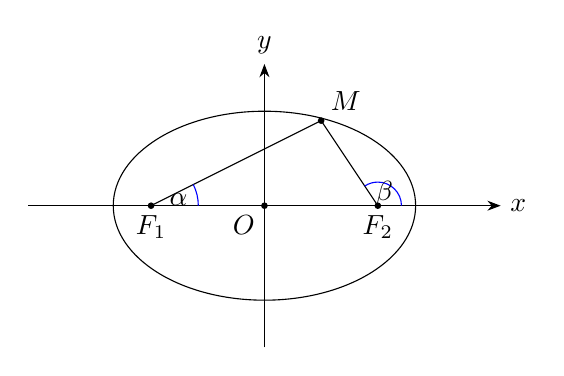
\begin{tikzpicture}[>=Stealth,scale=1.2]
        \coordinate (O) at (0,0);
        \coordinate (F1) at (-1.2,0);  % 不用下划线命名，避免和数学模式冲突
        \coordinate (F2) at (1.2,0);
        \coordinate (M) at (0.6,0.9);
        \coordinate (F3) at (2,0);
        \draw[->] (-2.5,0) -- (2.5,0) node[right] {$x$};
        \draw[->] (0,-1.5) -- (0,1.5) node[above] {$y$};
        \fill (0,0) circle (1pt) node[below left] {$O$};
        \fill (-1.2,0) circle (1pt) node[below] {$F_1$};
        \fill (1.2,0) circle (1pt) node[below] {$F_2$};
        \fill (0.6,0.9) circle (1pt) node[above right] {$M$};
        \draw (0,0) ellipse (1.6 and 1);
        \draw (-1.2,0) -- (0.6,0.9) -- (1.2,0);
        \pic [draw=blue, angle radius=0.6cm, "$\alpha$"] {angle=F2--F1--M};
        \pic [draw=blue, angle radius=0.3cm, "$\beta$"] {angle=F3--F2--M};
    \end{tikzpicture}
\end{center}


    \item \textbf{双曲线}：
    参数方程为 $\begin{cases} x = a\sec\varphi \\ y = b\tan\varphi \end{cases}$（$\varphi$ 为离心角），
    焦半径公式分左右支：
    \begin{itemize}
        \item 当点 $P$ 在右支上时：
        \begin{align*}
        |PF_1| &= \frac{b^2}{a-c \cos \theta},\\
        |PF_2| &= \frac{b^2}{a+c \cos \varphi }.
        \end{align*}
        \item 当点 $P$ 在左支上时：
        \begin{align*}
        |QF_1| &= \frac{b^2}{a-c \cos \gamma }, \\
        |QF_2| &= \frac{b^2}{a+c \cos \delta }.
        \end{align*}
    \end{itemize}
\end{enumerate}

\begin{center}
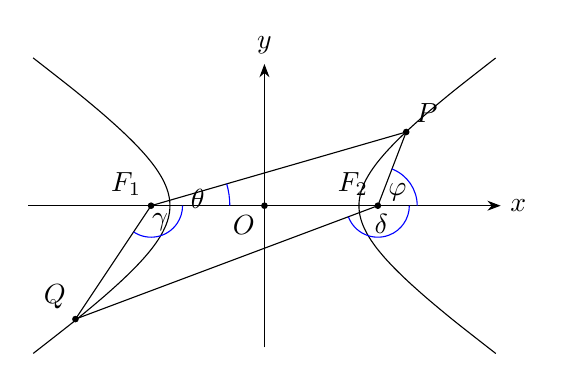
\begin{tikzpicture}[>=Stealth, scale=1.2]
    % ========== 1. 定义所有坐标点 ==========
    \coordinate (O) at (0,0);       % 原点
    \coordinate (F1) at (-1.2,0);   % 左焦点 F₁
    \coordinate (F2) at (1.2,0);    % 右焦点 F₂
    \coordinate (P) at (1.5,0.78);   % 双曲线上的点 M（右支）
    \coordinate (X) at (2,0);        % 辅助点：x轴正方向（用于标注β）
    \coordinate (Q) at (-2,-1.2);   % 双曲线上的点 Q（左支）
    % ========== 2. 画坐标轴 ==========
    \draw[->] (-2.5,0) -- (2.5,0) node[right] {$x$};
    \draw[->] (0,-1.5) -- (0,1.5) node[above] {$y$};

    % ========== 3. 画点并标注文字 ==========
    \fill (O) circle (1pt) node[below left] {$O$};
    \fill (F1) circle (1pt) node[above left] {$F_1$};
    \fill (F2) circle (1pt) node[above left] {$F_2$};
    \fill (P) circle (1pt) node[above right] {$P$};
    \fill (Q) circle (1pt) node[above left] {$Q$};

    % ========== 4. 画双曲线（核心修改：用参数方程绘制） ==========
    % 双曲线参数：设 a=1, c=1.2，则 b=√(c²-a²)≈0.66，这里取 b=0.7 方便绘图
    % 参数方程：x = a secθ, y = b tanθ（θ为离心角）
    \draw[domain=-1.15:1.15, smooth, variable=\t] 
        plot ({1/cos(\t r)}, {0.7*tan(\t r)}); % 右支
    \draw[domain=-1.15:1.15, smooth, variable=\t] 
        plot ({-1/cos(\t r)}, {-0.7*tan(\t r)}); % 左支

    % ========== 5. 画焦点三角形 F₁-M-F₂ ==========
    \draw (F1) -- (P) -- (F2);
    \draw (F1) -- (Q) -- (F2);
    % ========== 6. 标注夹角 α（∠MF₁F₂） ==========
    \pic [
        draw=blue,
        angle radius=1cm,
        "$\theta $"
    ] {angle=F2--F1--P};

    % ========== 7. 标注夹角 β（∠MF₂X，X为x轴正方向） ==========
    \pic [
        draw=blue,
        angle radius=0.5cm,
        "$\varphi $"
    ] {angle=X--F2--P};

    \pic [
        draw=blue,
        angle radius=0.4cm,
        "$\gamma  $"
    ] {angle=Q--F1--F2};

    \pic [
        draw=blue,
        angle radius=0.4cm,
        "$\delta   $"
    ] {angle=Q--F2--X};

\end{tikzpicture}
\end{center}
\end{tcolorbox}

\newpage

\begin{center}
    \subsection*{小节练习}
\end{center}
\vspace{2\baselineskip}

\noindent\textbf{例一： }已知双曲线的两个焦点$F_1\left(-\sqrt{10},0\right)$，$F_2\left(\sqrt{10},0\right)$，$M$是此双曲线上的一点，且$\overrightarrow{MF_1}\cdot\overrightarrow{MF_2}=0$，$\left|\overrightarrow{MF_1}\right|\cdot\left|\overrightarrow{MF_2}\right|=2$，则该双曲线的方程是 \hspace{1em} (\hspace{2em})
\par (A) $\dfrac{x^2}{9} - y^2 = 1$ \hspace{2em} (B) $x^2 - \dfrac{y^2}{9} = 1$
\par (C) $\dfrac{x^2}{9} - \dfrac{y^2}{7} = 1$ \hspace{2em} (D) $\dfrac{x^2}{7} - \dfrac{y^2}{3} = 1$
\vspace{2\baselineskip}

\noindent\textbf{例二： }(2018天津)已知双曲线$\dfrac{x^2}{a^2}-\dfrac{y^2}{b^2}=1\ (a>0,b>0)$的离心率为$2$，过右焦点且垂直于$x$轴的直线与双曲线交于$A,B$两点。设$A,B$到双曲线的同一条渐近线的距离分别为$d_1$和$d_2$，且$d_1+d_2=6$，则双曲线的方程是 \hspace{1em} (\hspace{2em})
\par (A) $\dfrac{x^2}{4} - \dfrac{y^2}{12} = 1$ \hspace{2em} (B) $\dfrac{x^2}{12} - \dfrac{y^2}{4} = 1$
\par (C) $\dfrac{x^2}{3} - \dfrac{y^2}{9} = 1$ \hspace{2em} (D) $\dfrac{x^2}{9} - \dfrac{y^2}{3} = 1$
\vspace{2\baselineskip}

\noindent\textbf{例三： }设双曲线与椭圆$\dfrac{x^2}{27}+\dfrac{y^2}{36}=1$有相同的焦点，且与椭圆相交，一个交点$A$的纵坐标为$4$，则此双曲线的方程为\underline{\hspace{5em}}。
\vspace{2\baselineskip}

\noindent\textbf{例四： }已知方程$\dfrac{x^2}{2+m}-\dfrac{y^2}{m+1}=1$表示双曲线，则$m$的取值范围为\underline{\hspace{5em}}。
\vspace{2\baselineskip}

\noindent\textbf{例五： }设椭圆$\dfrac{x^2}{a^2}+\dfrac{y^2}{b^2}=1\ (a>b>0)$与双曲线$\dfrac{x^2}{a^2}-\dfrac{y^2}{b^2}=1$的离心率分别为$e_1$，$e_2$，双曲线的渐近线的斜率小于$\dfrac{2\sqrt{5}}{5}$，则$e_1$的取值范围为\underline{\hspace{5em}}，$e_2$的取值范围为\underline{\hspace{5em}}。
\vspace{2\baselineskip}

\noindent\textbf{例六： }(2020全国一卷)设$F_1,F_2$是双曲线$C:x^2-\dfrac{y^2}{3}=1$的两个焦点，$O$为坐标原点，点$P$在$C$上且$|OP|=2$，则$\triangle PF_1F_2$的面积为\underline{\hspace{5em}}。
\vspace{2\baselineskip}

\noindent\textbf{例七： }(山东高考题改编)已知双曲线$E:\dfrac{x^2}{a^2}-\dfrac{y^2}{b^2}=1\ (a>0,b>0)$。若矩形$ABCD$的四个顶点都在$E$上，$AB,CD$的中点分别为$E$的两个焦点，且$2|AB|=3|BC|=6$，则$E$的标准方程是\underline{\hspace{5em}}。
\vspace{2\baselineskip}

\noindent\textbf{例八： }(新课标全国卷一)已知$F$是双曲线$C:x^2-\dfrac{y^2}{8}=1$的右焦点，$P$是$C$的左支上一点，$A\left(0,6\sqrt{6}\right)$。当$\triangle APF$周长最小时，该三角形的面积为\underline{\hspace{5em}}。
\vspace{2\baselineskip}

\noindent\textbf{例九： }(2022北京市海淀区模拟)已知$F_1,F_2$为双曲线$\dfrac{x^2}{a^2}-\dfrac{y^2}{b^2}=1\ (a>0,b>0)$的焦点，过$F_2$作垂直于$x$轴的直线交双曲线于点$P$，且$\angle PF_1F_2=30^\circ$，则双曲线的渐近线方程为\underline{\hspace{5em}}。
\vspace{2\baselineskip}

\noindent\textbf{例十： }(2019全国一卷)已知双曲线$C:\dfrac{x^2}{a^2}-\dfrac{y^2}{b^2}=1\ (a>0,b>0)$的左、右焦点分别为$F_1,F_2$，过$F_1$的直线与$C$的两条渐近线分别交于$A,B$两点。若$\overrightarrow{F_1A}=\overrightarrow{AB}$，$\overrightarrow{F_1B}\cdot\overrightarrow{F_2B}=0$，则$C$的离心率为\underline{\hspace{5em}}。
\vspace{2\baselineskip}

\noindent\textbf{例十一： }(2022上海)已知$P_1(x_1,y_1)$，$P_2(x_2,y_2)$两点均在双曲线$\Gamma:\dfrac{x^2}{a^2}-y^2=1\ (a>0)$的右支上，若$x_1x_2>y_1y_2$恒成立，则实数$a$的取值范围为\underline{\hspace{5em}}。
\vspace{2\baselineskip}

\noindent\textbf{例十二： }(课本原题)已知双曲线$x^2-\dfrac{y^2}{2}=1$，过点$P(1,1)$的直线$l$与双曲线相交于$A,B$两点，$P$能否是线段$AB$的中点？
\vspace{2\baselineskip}
 \vspace{2\baselineskip}
 \vspace{2\baselineskip}



\begin{tcolorbox}[colback=blue!10,colframe=blue!70!black,title=圆锥曲线的"垂"径定理]

\begin{center}
    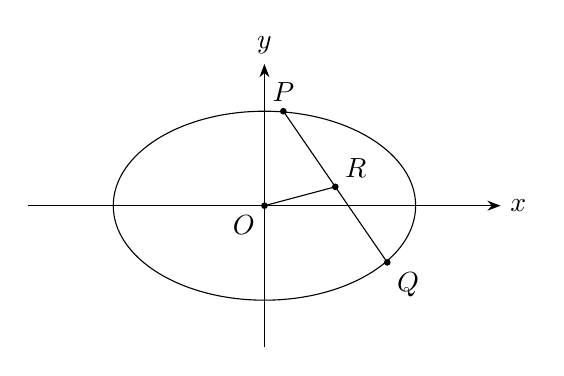
\begin{tikzpicture}[>=Stealth,scale=1.2]
        \coordinate (O) at (0,0);
        \coordinate (P) at (0.2,1);  % 不用下划线命名，避免和数学模式冲突
        \coordinate (Q) at (1.3,-0.6);
        \coordinate (R) at (0.75,0.2);

        \draw[->] (-2.5,0) -- (2.5,0) node[right] {$x$};
        \draw[->] (0,-1.5) -- (0,1.5) node[above] {$y$};
        
        \fill (0,0) circle (1pt) node[below left] {$O$};
        \fill (0.2,1) circle (1pt) node[above] {$P$};
        \fill (1.3,-0.6) circle (1pt) node[below right] {$Q$};
        \fill (0.75,0.2) circle (1pt) node[above right] {$R$};
        \draw (0,0) ellipse (1.6 and 1);
        \draw (0.2,1) -- (1.3,-0.6);
        \draw (0.75,0.2) -- (0,0);
        
    \end{tikzpicture}
\end{center}

如图所示，$P,Q$位于椭圆$\frac{x^2}{a^2}+\frac{y^2}{b^2}=1$上,若$R$为$PQ$的中点，则直线$PQ$与直线$RO$的斜率满足：

$$k_{PQ} \cdot k_{RO}=-\frac{b^2}{a^2}$$

\begin{center}
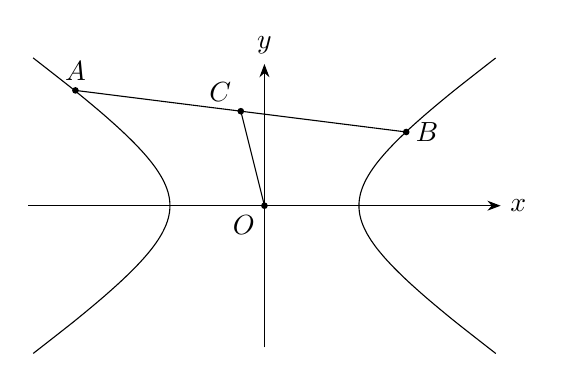
\begin{tikzpicture}[>=Stealth, scale=1.2]
    % ========== 1. 定义所有坐标点 ==========
    \coordinate (O) at (0,0);       % 原点
    \coordinate (A) at (-2,1.22);   % 左焦点 F₁
    \coordinate (B) at (1.5,0.78);   % 双曲线上的点 M（右支）
    \coordinate (X) at (2,0);        % 辅助点：x轴正方向（用于标注β）
    \coordinate (C) at (-0.25,1);   % 双曲线上的点 Q（左支）
    % ========== 2. 画坐标轴 ==========
    \draw[->] (-2.5,0) -- (2.5,0) node[right] {$x$};
    \draw[->] (0,-1.5) -- (0,1.5) node[above] {$y$};

    % ========== 3. 画点并标注文字 ==========
    \fill (O) circle (1pt) node[below left] {$O$};
    \fill (A) circle (1pt) node[above ] {$A$};
    \fill (B) circle (1pt) node[ right] {$B$};
    \fill (C) circle (1pt) node[above left] {$C$};

    \draw (A) -- (B);
    \draw (C) -- (O);
    % ========== 4. 画双曲线（核心修改：用参数方程绘制） ==========
    % 双曲线参数：设 a=1, c=1.2，则 b=√(c²-a²)≈0.66，这里取 b=0.7 方便绘图
    % 参数方程：x = a secθ, y = b tanθ（θ为离心角）
    \draw[domain=-1.15:1.15, smooth, variable=\t] 
        plot ({1/cos(\t r)}, {0.7*tan(\t r)}); % 右支
    \draw[domain=-1.15:1.15, smooth, variable=\t] 
        plot ({-1/cos(\t r)}, {-0.7*tan(\t r)}); % 左支

\end{tikzpicture}
\end{center}

如图所示，$A,B$位于双曲线$\frac{x^2}{a^2}-\frac{y^2}{b^2}=1$上,若$C$为$AB$的中点，则直线$AC$与直线$OB$的斜率满足：

$$k_{AC} \cdot k_{OB}=\frac{b^2}{a^2}$$


\end{tcolorbox}

\newpage

\subsection{抛物线}
 \vspace{2\baselineskip}


\textcolor{blue}{知识点1.}抛物线的定义及标准方程
 \vspace{2\baselineskip}

我们把平面内与一个定点 $F$ 和一条定直线 $l$（$l$ 不经过点 $F$）的距离相等的点的轨迹叫做抛物线. 点 $F$ 叫做抛物线的焦点, 直线 $l$ 叫做抛物线的准线.

根据抛物线焦点位置的不同, 抛物线的标准方程有以下四种不同的形式:
 \vspace{1\baselineskip}

\begin{center}
% 调整表格行高，避免内容与边线重合
\renewcommand{\arraystretch}{2.2}
% 固定列宽，保证每列空间充足，内容居中
\begin{tabular}{|m{2.2cm}|m{2.2cm}|m{2.2cm}|m{2.2cm}|m{2.2cm}|}
\hline
\centering 标准方程 & \centering $y^2 = 2px(p>0)$ & \centering $y^2 = -2px(p>0)$ & \centering $x^2 = 2py(p>0)$ & \centering $x^2 = -2py(p>0)$ \tabularnewline
\hline
\centering 图形 &
\centering
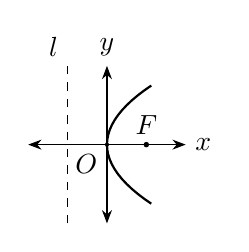
\begin{tikzpicture}[scale=0.5,>=Stealth,font=\normalsize]
% 双向坐标轴，符合教材样式
\draw[<->] (-2,0) -- (2,0) node[right]{$x$};
\draw[<->] (0,-2) -- (0,2) node[above]{$y$};
% 完整贯穿的准线虚线
\draw[dashed] (-1,-2) -- (-1,2) node[above left]{$l$};
% 焦点标注
\fill (1,0) circle (2pt) node[above]{$F$};
% 抛物线曲线
\draw[thick] plot[domain=-1.5:1.5] (0.5*\x*\x, \x);
% 原点标注
\fill (0,0) circle (1.5pt) node[below left]{$O$};
\end{tikzpicture}
&
\centering
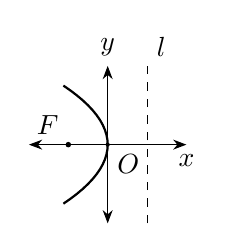
\begin{tikzpicture}[scale=0.5,>=Stealth,font=\normalsize]
\draw[<->] (-2,0) -- (2,0) node[below]{$x$};
\draw[<->] (0,-2) -- (0,2) node[above]{$y$};
\draw[dashed] (1,-2) -- (1,2) node[above right]{$l$};
\fill (-1,0) circle (2pt) node[above left]{$F$};
\draw[thick] plot[domain=-1.5:1.5] (-0.5*\x*\x, \x);
\fill (0,0) circle (1.5pt) node[below right]{$O$};
\end{tikzpicture}
&
\centering
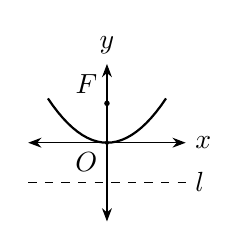
\begin{tikzpicture}[scale=0.5,>=Stealth,font=\normalsize]
% 双向坐标轴，和参考图完全匹配
\draw[<->] (-2,0) -- (2,0) node[right]{$x$};
\draw[<->] (0,-2) -- (0,2) node[above]{$y$};
% 完整的准线虚线，标注位置和参考图一致
\draw[dashed] (-2,-1) -- (2,-1) node[right]{$l$};
% 焦点位置与标注
\fill (0,1) circle (2pt) node[above left]{$F$};
% 开口向上的抛物线
\draw[thick] plot[domain=-1.5:1.5] (\x, 0.5*\x*\x);
% 原点标注
\fill (0,0) circle (1.5pt) node[below left]{$O$};
\end{tikzpicture}
&
\centering
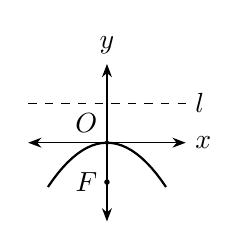
\begin{tikzpicture}[scale=0.5,>=Stealth,font=\normalsize]
\draw[<->] (-2,0) -- (2,0) node[right]{$x$};
\draw[<->] (0,-2) -- (0,2) node[above]{$y$};
% 准线在原点上方，和参考图一致
\draw[dashed] (-2,1) -- (2,1) node[right]{$l$};
% 焦点在y轴负半轴
\fill (0,-1) circle (2pt) node[left]{$F$};
% 开口向下的抛物线
\draw[thick] plot[domain=-1.5:1.5] (\x, -0.5*\x*\x);
% 原点标注
\fill (0,0) circle (1.5pt) node[above left]{$O$};
\end{tikzpicture}
\tabularnewline
\hline
\centering 焦点坐标 & \centering $\left(\frac{p}{2},0\right)$ & \centering $\left(-\frac{p}{2},0\right)$ & \centering $\left(0,\frac{p}{2}\right)$ & \centering $\left(0,-\frac{p}{2}\right)$ \tabularnewline
\hline
\centering 准线方程 & \centering $x = -\frac{p}{2}$ & \centering $x = \frac{p}{2}$ & \centering $y = -\frac{p}{2}$ & \centering $y = \frac{p}{2}$ \tabularnewline
\hline
\end{tabular}
\end{center}
 \vspace{1\baselineskip}

\begin{tcolorbox}[colback=blue!10,colframe=blue!70!black,title=]
\begin{enumerate}
    \item 只有抛物线的顶点在坐标原点，焦点在坐标轴上时，抛物线才具有标准形式。
    \item 标准方程的特征：等号的一边是某个变量的平方，等号的另一边是另一个变量的一次单项式。
    \item 焦点在 $y$ 轴上的抛物线的标准方程 $x^2 = \pm 2py(p>0)$ 通常又可以写成 $y=ax^2$，这与以前所学习的二次函数的解析式一致，但需要注意由方程 $y=ax^2$ 求焦点坐标和准线方程时，必须先将抛物线的方程化成标准形式。
\end{enumerate}
\end{tcolorbox}
 \vspace{1\baselineskip}

\textcolor{blue}{知识点2.}抛物线的焦半径公式

\begin{enumerate}
    \item 用坐标表示的焦半径公式

    由抛物线的定义可得到抛物线的焦半径公式如下：

    若点 $M(x_0,y_0)$ 是抛物线 $y^2 = 2px(p>0)$ 上一点，抛物线的焦点为 $F$，准线为 $l$，则线段 $MF$ 叫做抛物线的焦半径。如图 3.3.1-1 所示，过点 $M$ 作 $l$ 的垂线段 $MH$，由抛物线的定义可知 $|MF| = |MH| = x_0 + \frac{p}{2}$。

    \begin{center}
    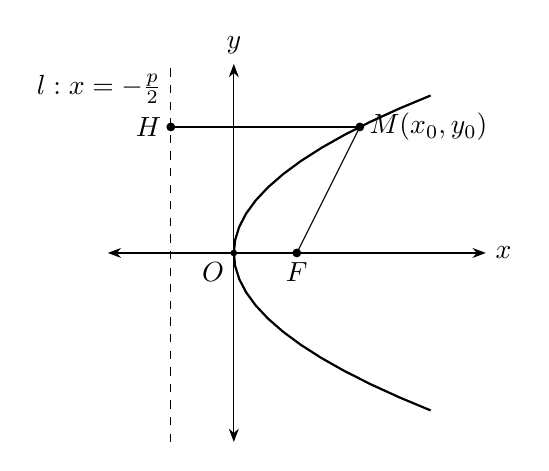
\begin{tikzpicture}[scale=0.8,>=Stealth,font=\normalsize]
    % 坐标轴
    \draw[<->] (-2,0) -- (4,0) node[right]{$x$};
    \draw[<->] (0,-3) -- (0,3) node[above]{$y$};
    % 准线
    \draw[dashed] (-1,-3) -- (-1,3) node[below left]{$l:x=-\frac{p}{2}$};
    % 焦点与原点
    \fill (1,0) circle (2pt) node[below]{$F$};
    \fill (0,0) circle (1.5pt) node[below left]{$O$};
    % 点M、H
    \coordinate (M) at (2,2);
    \coordinate (H) at (-1,2);
    \fill (M) circle (2pt) node[right]{$M(x_0,y_0)$};
    \fill (H) circle (2pt) node[left]{$H$};
    % 线段
    \draw (M) -- (H);
    \draw (M) -- (1,0);
    % 抛物线
    \draw[thick] plot[domain=-2.5:2.5] (0.5*\x*\x, \x);
    \end{tikzpicture}

    图1
    \end{center}

    同理可得，

    若点 $M(x_0,y_0)$ 在抛物线 $y^2 = -2px(p>0)$ 上，则 $|MF| = \frac{p}{2} - x_0$；

    若点 $M(x_0,y_0)$ 在抛物线 $x^2 = 2py(p>0)$ 上，则 $|MF| = y_0 + \frac{p}{2}$；

    若点 $M(x_0,y_0)$ 在抛物线 $x^2 = -2py(p>0)$ 上，则 $|MF| = \frac{p}{2} - y_0$。

    \item 用角 $\alpha$ 表示的焦半径公式

    如图2 所示，若倾斜角为 $\alpha$ 的直线 $AB$ 过抛物线 $y^2 = 2px(p>0)$ 的焦点 $F$，且与抛物线交于 $A,B$ 两点，则有:

    $$|AF| = \frac{p}{1-\cos\alpha}\;\;\;\;\;\;\;\;\;\;|BF| = \frac{p}{1+\cos\alpha}$$

    证明如下：

    如图2 所示，设 $A,B$ 在准线 $l$ 与 $x$ 轴上的射影分别为 $C,D$ 和 $E,G$，准线 $l$ 与 $x$ 轴交于 $P$ 点，则有
    $$|AF| = |AC| = |EP| = |PF| + |EF| = |PF| + |AF|\cos\alpha,$$
    所以 $|AF| = \frac{p}{1-\cos\alpha}$，同理可得 $|BF| = \frac{p}{1+\cos\alpha}$。

    \begin{center}
    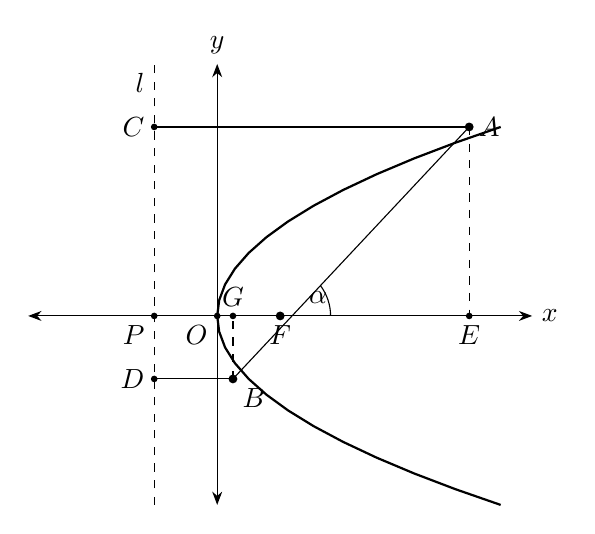
\begin{tikzpicture}[scale=0.8,>=Stealth,font=\normalsize]
    % 坐标轴
    \draw[<->] (-3,0) -- (5,0) node[right]{$x$};
    \draw[<->] (0,-3) -- (0,4) node[above]{$y$};
    % 准线与点P
    \draw[dashed] (-1,-3) -- (-1,4) node[below left]{$l$};
    \fill (-1,0) circle (1.5pt) node[below left]{$P$};
    % 原点与焦点
    \fill (0,0) circle (1.5pt) node[below left]{$O$};
    \fill (1,0) circle (2pt) node[below]{$F$};
    % 点A及射影C、E
    \coordinate (A) at (4,3);
    \coordinate (C) at (-1,3);
    \coordinate (E) at (4,0);
    \fill (A) circle (2pt) node[right]{$A$};
    \fill (C) circle (1.5pt) node[left]{$C$};
    \fill (E) circle (1.5pt) node[below]{$E$};
    \draw (A) -- (C);
    \draw[dashed] (A) -- (E);
    % 点B及射影D、G
    \coordinate (B) at (0.25,-1);
    \coordinate (D) at (-1,-1);
    \coordinate (G) at (0.25,0);
    \fill (B) circle (2pt) node[below right]{$B$};
    \fill (D) circle (1.5pt) node[left]{$D$};
    \fill (G) circle (1.5pt) node[above]{$G$};
    \draw (B) -- (D);
    \draw[dashed] (B) -- (G);
    % 直线AB与倾斜角
    \draw (A) -- (B);
    \draw (1,0) ++(0.8,0) arc (0:37:0.8);
    \node at (1.6,0.3) {$\alpha$};
    % 抛物线
    \draw[thick] plot[domain=-3:3] (0.5*\x*\x, \x);
    \end{tikzpicture}

    图2
    \end{center}

\end{enumerate}
 \vspace{1\baselineskip}

\textcolor{blue}{知识点3.}抛物线的简单几何性质

 \vspace{1\baselineskip}

\begin{center}
% 调整表格行高，避免内容拥挤
\renewcommand{\arraystretch}{2.2}
\begin{tabular}{|c|c|c|c|c|c|}
\hline
\multicolumn{2}{|c|}{标准方程} & $y^2 = 2px(p>0)$ & $y^2 = -2px(p>0)$ & $x^2 = 2py(p>0)$ & $x^2 = -2py(p>0)$ \\
\hline
\multicolumn{2}{|c|}{图形} &
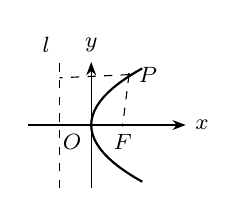
\begin{tikzpicture}[scale=0.4,>=Stealth,font=\footnotesize]
\draw[->] (-2,0) -- (3,0) node[right]{$x$};
\draw[->] (0,-2) -- (0,2) node[above]{$y$};
\draw[dashed] (-1,-2) -- (-1,2) node[above left]{$l$};
\fill (1,0) circle (1.5pt) node[below]{$F$};
\fill (0,0) circle (1pt) node[below left]{$O$};
\coordinate (P) at (1.2,1.6);
\fill (P) circle (1.5pt) node[right]{$P$};
\draw[dashed] (P) -- (-1,1.5);
\draw[dashed] (P) -- (1,0);
\draw[thick] plot[domain=-1.8:1.8] (0.5*\x*\x, \x);
\end{tikzpicture}
&
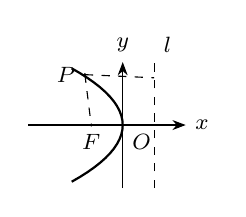
\begin{tikzpicture}[scale=0.4,>=Stealth,font=\footnotesize]
\draw[->] (-3,0) -- (2,0) node[right]{$x$};
\draw[->] (0,-2) -- (0,2) node[above]{$y$};
\draw[dashed] (1,-2) -- (1,2) node[above right]{$l$};
\fill (-1,0) circle (1.5pt) node[below]{$F$};
\fill (0,0) circle (1pt) node[below right]{$O$};
\coordinate (P) at (-1.2,1.6);
\fill (P) circle (1.5pt) node[left]{$P$};
\draw[dashed] (P) -- (1,1.5);
\draw[dashed] (P) -- (-1,0);
\draw[thick] plot[domain=-1.8:1.8] (-0.5*\x*\x, \x);
\end{tikzpicture}
&
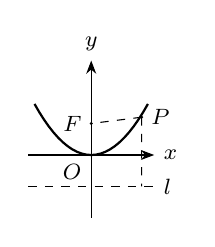
\begin{tikzpicture}[scale=0.4,>=Stealth,font=\footnotesize]
\draw[->] (-2,0) -- (2,0) node[right]{$x$};
\draw[->] (0,-2) -- (0,3) node[above]{$y$};
\draw[dashed] (-2,-1) -- (2,-1) node[right]{$l$};
\fill (0,1) circle (1.5pt) node[left]{$F$};
\fill (0,0) circle (1pt) node[below left]{$O$};
\coordinate (P) at (1.6,1.2);
\fill (P) circle (1.5pt) node[right]{$P$};
\draw[dashed] (P) -- (1.6,-1);
\draw[dashed] (P) -- (0,1);
\draw[thick] plot[domain=-1.8:1.8] (\x, 0.5*\x*\x);
\end{tikzpicture}
&
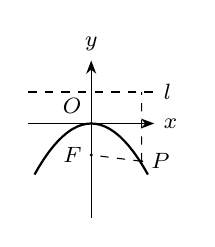
\begin{tikzpicture}[scale=0.4,>=Stealth,font=\footnotesize]
\draw[->] (-2,0) -- (2,0) node[right]{$x$};
\draw[->] (0,-3) -- (0,2) node[above]{$y$};
\draw[dashed] (-2,1) -- (2,1) node[right]{$l$};
\fill (0,-1) circle (1.5pt) node[left]{$F$};
\fill (0,0) circle (1pt) node[above left]{$O$};
\coordinate (P) at (1.6,-1.2);
\fill (P) circle (1.5pt) node[right]{$P$};
\draw[dashed] (P) -- (1.6,1);
\draw[dashed] (P) -- (0,-1);
\draw[thick] plot[domain=-1.8:1.8] (\x, -0.5*\x*\x);
\end{tikzpicture}
\\
\hline
\multirow{4}{*}{\rotatebox{90}{几何性质}} & 范围 & $x\geq0,y\in\mathbf{R}$ & $x\leq0,y\in\mathbf{R}$ & $y\geq0,x\in\mathbf{R}$ & $y\leq0,x\in\mathbf{R}$ \\
\cline{2-6}
& 对称性 & \multicolumn{2}{c|}{关于$x$轴对称} & \multicolumn{2}{c|}{关于$y$轴对称} \\
\cline{2-6}
& 顶点 & \multicolumn{4}{c|}{坐标原点} \\
\cline{2-6}
& 离心率 & \multicolumn{4}{c|}{$e=1$} \\
\hline
\end{tabular}
\end{center}
 \vspace{1\baselineskip}

\textcolor{blue}{知识点4.}直线与抛物线的关系
 \vspace{1\baselineskip}

直线与抛物线有三种位置关系：相离、相切、相交。（以抛物线 $y^2 = 2px$ 为例说明）

\begin{enumerate}[label=(\arabic*)]
    \item 直线的斜率存在时，

    设直线 $l:y = kx + m$。将 $y = kx + m$ 代入 $y^2 = 2px$，消去 $y$ 并化简，得
    $$k^2x^2 + 2(mk - p)x + m^2 = 0.$$

    \begin{enumerate}
        \item 当 $k = 0$ 时，直线平行于抛物线的对称轴或与对称轴重合，直线与抛物线只有一个公共点。
        \item 当 $k \neq 0$ 时，

        判别式 $\Delta > 0 \Leftrightarrow$ 直线与抛物线相交，有两个公共点；

        判别式 $\Delta = 0 \Leftrightarrow$ 直线与抛物线相切，有且只有一个公共点；

        判别式 $\Delta < 0 \Leftrightarrow$ 直线与抛物线相离，没有公共点。
    \end{enumerate}

    \item 直线的斜率不存在时，

    设直线 $l:x = m$。

    显然，当 $m < 0$ 时，直线与抛物线相离，无交点；

    当 $m = 0$ 时，直线与抛物线相切，有一个交点；

    当 $m > 0$ 时，直线与抛物线相交，有两个交点。
\end{enumerate}
 \vspace{2\baselineskip}

\begin{center}
\subsection*{微专题：抛物线焦点弦性质的探究及拓展}
\end{center}

\subsubsection*{1 焦点弦的常用性质}

\;\;\;\;\;\;如图 3，$AB$ 是抛物线 $y^2 = 2px(p>0)$ 过焦点 $F$ 的一条弦，直线 $AB$ 的倾斜角为 $\theta$，设 $A(x_1,y_1),B(x_2,y_2)$，过 $A,B$ 分别向抛物线的准线作垂线，垂足分别为 $A_1,B_1$，$E$ 为准线与 $x$ 轴的交点。对于抛物线的焦点弦，有如下结论：

\begin{center}
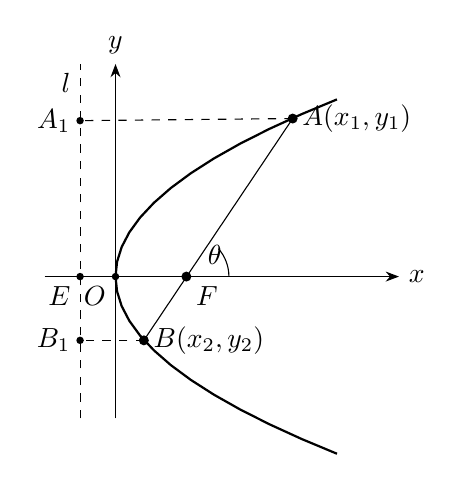
\begin{tikzpicture}[scale=0.9,>=Stealth,font=\normalsize]
% 坐标轴
\draw[->] (-1,0) -- (4,0) node[right]{$x$};
\draw[->] (0,-2) -- (0,3) node[above]{$y$};
% 准线与E点
\draw[dashed] (-0.5,-2) -- (-0.5,3) node[below left]{$l$};
\fill (-0.5,0) circle (1.5pt) node[below left]{$E$};
% 原点、焦点
\fill (0,0) circle (1.5pt) node[below left]{$O$};
\fill (1,0) circle (2pt) node[below right]{$F$};
% 点A、A1
\coordinate (A) at (2.5,2.23);
\coordinate (A1) at (-0.5,2.2);
\fill (A) circle (2pt) node[right]{$A(x_1,y_1)$};
\fill (A1) circle (1.5pt) node[left]{$A_1$};
\draw[dashed] (A) -- (A1);
% 点B、B1
\coordinate (B) at (0.4,-0.9);
\coordinate (B1) at (-0.5,-0.9);
\fill (B) circle (2pt) node[right]{$B(x_2,y_2)$};
\fill (B1) circle (1.5pt) node[left]{$B_1$};
\draw[dashed] (B) -- (B1);
% 直线AB
\draw (A) -- (B);
% 倾斜角θ
\draw (1,0) ++(0.6,0) arc (0:41:0.6);
\node at (1.4,0.3) {$\theta$};
% 抛物线
\draw[thick] plot[domain=-2.5:2.5] (0.5*\x*\x, \x);
\end{tikzpicture}

图 3
\end{center}

\begin{enumerate}
    \item $x_1x_2 = \dfrac{p^2}{4}$，$y_1y_2 = -p^2$。
    \item 若 $A$ 位于 $x$ 轴上方，$B$ 位于 $x$ 轴下方，则 $|AF| = \dfrac{p}{1-\cos\theta}$，$|BF| = \dfrac{p}{1+\cos\theta}$。

    证明：$|AF| = |AA_1| = |EF| + |AF|\cos\theta = p + |AF|\cdot\cos\theta$，$\therefore |AF| = \dfrac{p}{1-\cos\theta}$，同理，$|BF| = \dfrac{p}{1+\cos\theta}$。
    \item $|AB| = x_1 + x_2 + p = \dfrac{2p}{\sin^2\theta}$，抛物线的通径（过抛物线的焦点作垂直于对称轴而交抛物线于 $A,B$ 两点的线段 $AB$，称为抛物线的通径）长为 $2p$，通径是最短的焦点弦。
    \item $S_{\triangle AOB} = \dfrac{p^2}{2\sin\theta}$。
    \item $\dfrac{1}{|AF|} + \dfrac{1}{|BF|} = \dfrac{2}{p}$，$\dfrac{|AF|}{|BF|} = \dfrac{1+\cos\theta}{1-\cos\theta}$。
    \item 设弦 $AB$ 所在直线的斜率为 $k$，则焦点弦长的斜率式为 $|AB| = 2p\left(1 + \dfrac{1}{k^2}\right)$。
\end{enumerate}

\subsubsection*{2 与焦点弦有关的切线性质}

\;\;\;\;\;\;如图 4，$AB$ 是抛物线 $x^2 = 2py(p>0)$ 过焦点的一条弦，分别过 $A,B$ 作抛物线的切线，两切线交于点 $P$，连接 $PF$，则有以下结论：

\begin{center}
\begin{tikzpicture}[scale=1.2,>=Stealth,font=\small]
    % 取 p = 2，焦点 F(0,1)，准线 l:y=-1（严格对称）
    \def\p{2}
    \def\halfp{1} % 用整数代替小数，避免运算报错

    % 坐标轴与原点
    \draw[->] (-4,0) -- (4,0) node[right]{$x$};
    \draw[->] (0,-2.5) -- (0,3.5) node[above]{$y$};
    \fill (0,0) circle (1.2pt) node[below left]{$O$};

    % 焦点 F（0,1），到原点距离=1
    \fill (0,\halfp) circle (1.5pt) node[above left]{$F$};

    % 准线 l:y=-1（到原点距离=1，与焦点严格对称）
    \draw[dashed] (-4,-\halfp) -- (4,-\halfp) node[right]{$l$};

    % 准线上取点 P(1,-1)
    \coordinate (P) at (1,-\halfp);
    \fill (P) circle (1.5pt) node[below right]{$P$};

    % 抛物线 x²=4y，即 y = x²/4
    \draw[thick] plot[domain=-3.5:3.5] (\x, {0.25*\x*\x});

    % 用具体数值代替根号运算，避免编译报错
    % A ≈ (1-√5, (6-2√5)/4) ≈ (-1.236, 0.382)
    \coordinate (A) at (-1.236, 0.382);
    % B ≈ (1+√5, (6+2√5)/4) ≈ (3.236, 2.618)
    \coordinate (B) at (3.236, 2.618);

    % 标注切点
    \fill (A) circle (1.5pt) node[above left]{$A$};
    \fill (B) circle (1.5pt) node[above right]{$B$};

    % 切线 PA、PB（严格相切）
    \draw[thick] (A) -- (P);
    \draw[thick] (B) -- (P);

    % 焦点弦 AB（F 严格在线段 AB 上）
    \draw[thick] (A) -- (B);

    % 辅助线 PF
    \draw[dashed] (P) -- (0,\halfp);
\end{tikzpicture}

图 4
\end{center}

\begin{enumerate}[label=\textcircled{\arabic*}]
    \item 点 $P$ 的轨迹是一条直线，即抛物线的准线 $l:y = -\dfrac{p}{2}$。
    \item 两切线互相垂直，即 $PA \perp PB$。
    \item $PF \perp AB$。
    \item 点 $P$ 的坐标为 $\left( \dfrac{x_A + x_B}{2}, -\dfrac{p}{2} \right)$。
\end{enumerate}

\subsubsection*{3 非焦点弦性质}

\begin{enumerate}[label=\textcircled{\arabic*}]
    \item 已知直线 $l$ 与抛物线 $y^2 = 2px(p>0)$ 交于 $A,B$ 两点，若 $OA \perp OB$，则直线 $l$ 过定点 $(2p,0)$，反之亦成立。
    \item 已知 $M(x_0,y_0)$ 是抛物线 $y^2 = 2px(p>0)$ 上任意一点，点 $N(a,0)$ 是抛物线的对称轴上一点，则
    $$|MN|_{\text{min}} =
    \begin{cases}
    |a| & (a \leqslant p), \\
    \sqrt{2pa - p^2} & (a > p).
    \end{cases}$$
\end{enumerate}

\subsubsection*{4 抛物线几何性质的深挖}

\;\;\;\;\;\;如图 5 所示，设过抛物线 $y^2 = 2px(p>0)$ 焦点 $F$ 的直线与抛物线交于 $A,B$ 两点，过 $A,B$ 两点作准线 $l$ 的垂线，垂足分别为 $A',B'$，$N$ 为 $l$ 与 $x$ 轴的交点。连接 $A'F$，$B'F$，由抛物线的定义可知 $|AF| = |AA'|$，$|BF| = |BB'|$，所以 $\angle AFA' = \angle AA'F$，$\angle BFB' = \angle BB'F$。又 $AA' \perp l$，$x$ 轴 $\perp l$，$\therefore \angle AA'F = \angle A'FN$。同理 $\angle BB'F = \angle B'FN$，$\therefore \angle A'FB' = 90^\circ$，即 $A'F \perp B'F$。$\cdots\cdots$（结论 1）

\begin{center}
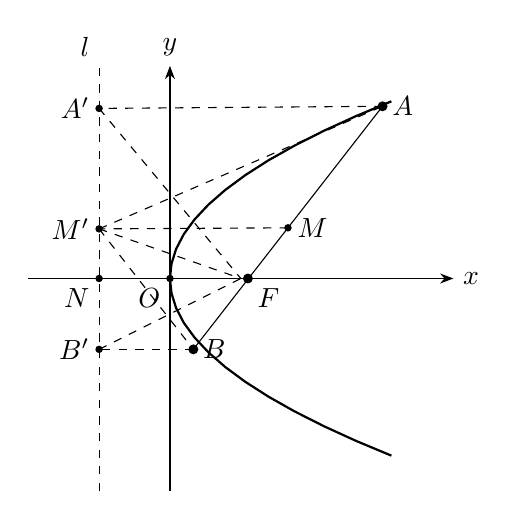
\begin{tikzpicture}[scale=0.9,>=Stealth,font=\normalsize]
% 坐标轴
\draw[->] (-2,0) -- (4,0) node[right]{$x$};
\draw[->] (0,-3) -- (0,3) node[above]{$y$};
% 准线l与N点
\draw[dashed] (-1,-3) -- (-1,3) node[above left]{$l$};
\fill (-1,0) circle (1.5pt) node[below left]{$N$};
% 原点、焦点
\fill (0,0) circle (1.5pt) node[below left]{$O$};
\fill (1.1,0) circle (2pt) node[below right]{$F$};
% 点A、A'
\coordinate (A) at (3,2.43);
\coordinate (A') at (-1,2.4);
\fill (A) circle (2pt) node[right]{$A$};
\fill (A') circle (1.5pt) node[left]{$A'$};
\draw[dashed] (A) -- (A');
% 点B、B'
\coordinate (B) at (0.33,-1);
\coordinate (B') at (-1,-1);
\fill (B) circle (2pt) node[right]{$B$};
\fill (B') circle (1.5pt) node[left]{$B'$};
\draw[dashed] (B) -- (B');
% 直线AB
\draw (A) -- (B);
% 中点M、M'
\coordinate (M) at ($(A)!0.5!(B)$);
\coordinate (M') at (-1,0.7);
\fill (M) circle (1.5pt) node[right]{$M$};
\fill (M') circle (1.5pt) node[left]{$M'$};
\draw[dashed] (M) -- (M');
% 辅助线
\draw[dashed] (A') -- (1,0);
\draw[dashed] (B') -- (1,0);
\draw[dashed] (M') -- (1,0);
\draw[dashed] (M') -- (A);
\draw[dashed] (M') -- (B);
% 抛物线
\draw[thick] plot[domain=-2.5:2.5] (0.5*\x*\x, \x);
\end{tikzpicture}

图 5
\end{center}

\;\;\;\;\;\;设 $AB$ 和 $A'B'$ 的中点分别为 $M,M'$，连接 $MM',M'F$，则 $\angle M'FA' = \angle M'A'F$。$\therefore \angle M'FA = \angle M'FB = 90^\circ$，即 $M'F \perp AB$。$\cdots\cdots$（结论 2）

\;\;\;\;\;\;$\therefore A,A',M',F$ 四点共圆，且 $B,B',M',F$ 四点共圆。$\cdots\cdots$（结论 3）

\;\;\;\;\;\;由于 $|MM'| = \dfrac{1}{2}(|AA'| + |BB'|) = \dfrac{1}{2}(|AF| + |BF|) = \dfrac{1}{2}|AB|$，即 $M$ 到 $l$ 的距离等于 $|AB|$ 的一半，所以以 $AB$ 为直径的圆与 $l$ 相切于点 $M'$。$\cdots\cdots$（结论 4）

\;\;\;\;\;\;同理可证以 $AF$ 为直径的圆与 $y$ 轴相切，以 $BF$ 为直径的圆也与 $y$ 轴相切。$\cdots\cdots$（结论 5）

\;\;\;\;\;\;连接 $AM',BM'$，在 $\triangle AM'B$ 中，$AM = BM = MM'$，则 $\angle AM'B = 90^\circ$，即 $AM' \perp BM'$。$\cdots\cdots$（结论 6）

\subsubsection*{5 过抛物线对称轴上一定点的弦的性质的深挖}

\;\;\;\;\;\;我们知道，抛物线 $y^2 = 2px(p>0)$ 的焦点弦 $AB$（其中 $A(x_1,y_1),B(x_2,y_2)$）有性质 $y_1y_2 = -p^2$（为定值），那么过点 $(a,0)$ 的直线 $l$ 与抛物线交于两点 $(x_1,y_1)$，$(x_2,y_2)$，是否也有类似的性质呢？

\;\;\;\;\;\;设直线 $l$ 的方程为 $x = ty + a$，
与 $y^2 = 2px(p>0)$ 联立，得 $y^2 - 2pty - 2pa = 0$，所以 $y_1y_2 = -2pa$（为定值）。$\cdots\cdots$（结论 7）

\;\;\;\;\;\;于是 $x_1x_2 = \dfrac{y_1^2}{2p} \cdot \dfrac{y_2^2}{2p} = \dfrac{4p^2a^2}{4p^2} = a^2$（为定值）。$\cdots\cdots$（结论 8）

\;\;\;\;\;\;$k_{OA}k_{OB} = \dfrac{y_1}{x_1} \cdot \dfrac{y_2}{x_2} = \dfrac{y_1}{\dfrac{y_1^2}{2p}} \cdot \dfrac{y_2}{\dfrac{y_2^2}{2p}} = \dfrac{4p^2}{y_1y_2} = -\dfrac{2p}{a}$（为定值）。$\cdots\cdots$（结论 9）

\;\;\;\;\;\;反过来，若 $y_1y_2 = -2pa$（为定值），则直线 $l$ 是否过定点呢？
设直线 $l$ 的方程为 $x = t'y + a'$，与 $y^2 = 2px$ 联立得 $y^2 - 2pt'y - 2pa' = 0$，所以 $y_1y_2 = -2pa' = -2pa$，所以 $a' = a$，即直线 $l$ 过定点 $(a,0)$。$\cdots\cdots$（结论 10）
\vspace{3em}

\noindent
\textbf{例题: }（新高考一卷）已知$F$为抛物线$C:y^2 = 4x$的焦点，过$F$作两条互相垂直的直线$l_1$，$l_2$，直线$l_1$与$C$交于$A$，$B$两点，直线$l_2$与$C$交于$D$，$E$两点，则$|AB| + |DE|$的最小值为
\vspace{0.5em}

A. $16$ \quad
B. $14$ \quad
C. $12$ \quad
D. $10$

\newpage

\begin{center}
    \subsection*{小节练习}
\end{center}

\textbf{例一：}（2020全国一卷）已知$A$为抛物线$C:y^2=2px(p>0)$上一点，点$A$到$C$的焦点的距离为12，到$y$轴的距离为9，则$p=$
\vspace{0.5em}

A. $2$ \quad B. $3$ \quad C. $6$ \quad D. $9$
\vspace{2\baselineskip}

\textbf{例二：}（2020北京）设抛物线的顶点为$O$，焦点为$F$，准线为$l$，$P$是抛物线上异于$O$的一点，过$P$作$PQ \perp l$于$Q$。则线段$FQ$的垂直平分线
\vspace{0.5em}

A. 经过点$O$ \quad B. 经过点$P$ \quad C. 平行于直线$OP$ \quad D. 垂直于直线$OP$
\vspace{2\baselineskip}

\textbf{例三：}（浙江高考题）设抛物线$y^2=4x$的焦点为$F$，不经过焦点的直线上有三个不同的点$A,B,C$，其中点$A,B$在抛物线上，点$C$在$y$轴上，则$\triangle BCF$与$\triangle ACF$的面积之比是
\vspace{0.5em}

A. $\dfrac{|BF|-1}{|AF|-1}$ \quad B. $\dfrac{|BF|^2-1}{|AF|^2-1}$ \quad C. $\dfrac{|BF|+1}{|AF|+1}$ \quad D. $\dfrac{|BF|^2+1}{|AF|^2+1}$
\begin{center}
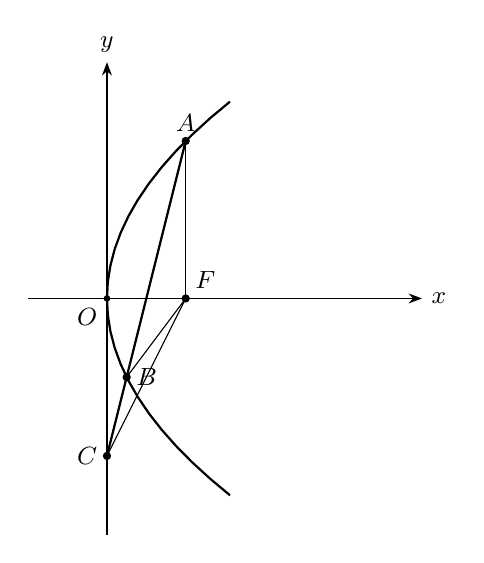
\begin{tikzpicture}[scale=1,>=Stealth,font=\small]
    % ========== 第一步：严格计算坐标，保证几何关系 ==========
    % 抛物线 y²=4x，焦点F(1,0)
    \coordinate (O) at (0,0);
    \coordinate (F) at (1,0);
    
    % 严格取点：
    % A(1, 2) 在抛物线上 (2²=4*1)
    % B(0.25, -1) 在抛物线上 ((-1)²=4*0.25)
    % 直线AB方程：y = 4x - 2
    % C(0, -2) 是直线AB与y轴的交点
    % 因此 A、B、C 严格共线
    \coordinate (A) at (1,2);
    \coordinate (B) at (0.25,-1);
    \coordinate (C) at (0,-2);

    % ========== 第二步：画坐标轴、抛物线 ==========
    \draw[->] (-1,0) -- (4,0) node[right]{$x$};
    \draw[->] (0,-3) -- (0,3) node[above]{$y$};
    \draw[thick] plot[domain=-2.5:2.5] (\x*\x/4, \x);

    % ========== 第三步：标注点 ==========
    \fill (O) circle (1.2pt) node[below left]{$O$};
    \fill (F) circle (1.5pt) node[above right]{$F$};
    \fill (A) circle (1.5pt) node[above]{$A$};
    \fill (B) circle (1.5pt) node[ right]{$B$};
    \fill (C) circle (1.5pt) node[left]{$C$};

    % ========== 第四步：连线（A-B-C严格共线） ==========
    \draw[thick] (C) -- (A); % 画一条直线穿过C、B、A
    \draw (C) -- (F);
    \draw (A) -- (F);
    \draw (B) -- (F);

\end{tikzpicture}
\end{center}
\vspace{2\baselineskip}

\textbf{例四：}（2022浙江省台州市期末）在正方体$ABCD - A_1B_1C_1D_1$中，$P$是侧面$BB_1C_1C$内一动点，若点$P$到直线$BC$与直线$C_1D_1$的距离相等，则动点$P$的轨迹所在的曲线是
\vspace{0.5em}

A. 直线 \quad B. 圆 \quad C. 椭圆 \quad D. 抛物线

\begin{center}
    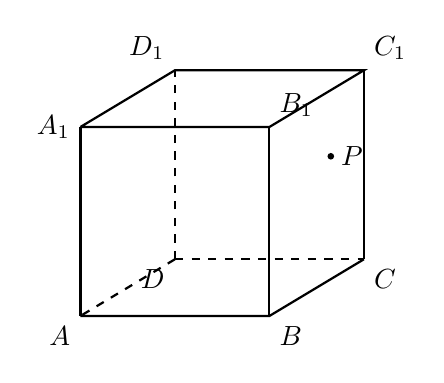
\begin{tikzpicture}[
    % 斜二测视角，完全匹配教材正方体的画法
    x={(1cm, 0cm)},
    y={(0.5cm, 0.3cm)},
    z={(0cm, 1cm)},
    font=\normalsize,
    scale=0.6,
    thick
]

% 定义正方体顶点坐标（边长为4，适配标注位置）
\coordinate (A) at (0, 0, 0);
\coordinate (B) at (4, 0, 0);
\coordinate (C) at (4, 4, 0);
\coordinate (D) at (0, 4, 0);
\coordinate (A1) at (0, 0, 4);
\coordinate (B1) at (4, 0, 4);
\coordinate (C1) at (4, 4, 4);
\coordinate (D1) at (0, 4, 4);
% P点位置：右侧面BCC₁B₁内部，和原图位置完全匹配
\coordinate (P) at (4, 2.6, 2.6);

% 第一步：绘制不可见的虚线棱（被遮挡的部分）
\draw[dashed] (D) -- (D1);
\draw[dashed] (D) -- (C);
\draw[dashed] (D) -- (A);

% 第二步：绘制可见的实线棱
% 底面可见边
\draw (A) -- (B) -- (C);
% 顶面完整边
\draw (A1) -- (B1) -- (C1) -- (D1) -- (A1);
% 竖棱
\draw (A) -- (A1);
\draw (B) -- (B1);
\draw (C) -- (C1);

% 第三步：标注顶点，位置和原图完全对应
\node at (A) [below left] {$A$};
\node at (B) [below right] {$B$};
\node at (C) [below right] {$C$};
\node at (D) [below left] {$D$};
\node at (A1) [left] {$A_1$};
\node at (B1) [above right] {$B_1$};
\node at (C1) [above right] {$C_1$};
\node at (D1) [above left] {$D_1$};

% 第四步：绘制P点并标注
\fill (P) circle (2pt) node[right] {$P$};

\end{tikzpicture}

\end{center}

\textbf{例五：} 垂直于$x$轴的直线交抛物线$y^2=4x$于$A$，$B$两点，且$|AB|=4\sqrt{3}$，则直线$AB$的方程为$\underline{\qquad\qquad\qquad\qquad}$ 
\vspace{2\baselineskip}

\textbf{例六：} 已知圆心在$y$轴上移动的圆经过点$A(0,5)$，且与$x$轴、$y$轴分别交于$B(x,0)$，$C(0,y)$两个动点，则点$M(x,y)$的轨迹方程为$\underline{\qquad\qquad\qquad\qquad}$ 
\vspace{2\baselineskip}

\textbf{例七：} 如图，已知直线与抛物线$y^2=2px(p>0)$交于$A$，$B$两点，且$OA \perp OB$，$OD \perp AB$交$AB$于点$D$，点$D$的坐标为$(2,1)$，则$p$的值为$\underline{\qquad\qquad}$ 
\vspace{2\baselineskip}

\textbf{例八：}（2021北京）已知抛物线$C:y^2=4x$，$C$的焦点为$F$，点$M$在$C$上，且$|FM|=6$，则点$M$的横坐标是$\underline{\qquad\qquad}$ 
\vspace{2\baselineskip}

\textbf{例九：}（2021新高考二卷）已知$O$为坐标原点，抛物线$C:y^2=2px(p>0)$的焦点为$F$，$P$为$C$上一点，$PF$与$x$轴垂直，$Q$为$x$轴上一点，且$PQ \perp OP$。若$|FQ|=6$，则$C$的准线方程为$\underline{\qquad\qquad\qquad\qquad}$ 
\vspace{2\baselineskip}

\newpage

\section{题型专练}
\subsection{直线与圆综合问题（小题）}

\noindent\textbf{例一： }(2019·河西三模)垂直于直线 $y=x+1$ 且与圆 $x^2+y^2=1$ 相切于第一象限的直线方程是$\underline{\qquad\qquad\qquad\qquad}$   \vspace{2\baselineskip}

% 例2
\noindent\textbf{例二： }求圆 $x^2+y^2-10x-10y=0$ 与圆 $x^2+y^2-6x+2y-40=0$ 的公共弦长.   \vspace{2\baselineskip}

% 例3
\noindent\textbf{例三： }(2023·河西一模)与直线 $x-y-4=0$ 和圆 $C:x^2+y^2+2x-2y=0$ 都相切的半径最小的圆的方程是$\underline{\qquad\qquad\qquad\qquad}$   \vspace{2\baselineskip}

% 例4
\noindent\textbf{例四： }(2022·和平一模)已知圆 $C$ 的圆心在直线 $2x-y-2=0$ 上，且与直线 $l:3x+4y-28=0$ 相切于点 $P(4,4)$，则圆 $C$ 的标准方程为$\underline{\qquad\qquad\qquad\qquad}$   \vspace{2\baselineskip}

% 例5
\noindent\textbf{例五： }(2022·福建一中期中)已知圆 $x^2+y^2=36$ 与圆 $(x-10)^2+y^2=64$ 交于 $A,B$ 两点，$A$ 在第一象限，则 $|AB|=\underline{\qquad}$；若过点 $A$ 的弦交两圆于 $C,D$ 两点，且 $|AC|=|AD|$，则直线 $CD$ 的斜率是$\underline{\qquad}$.   \vspace{2\baselineskip}

% 例6
\noindent\textbf{例六： }求由曲线 $x^2+y^2=|x|+|y|$ 围成的图形的面积.   \vspace{2\baselineskip}

% 例7
\noindent\textbf{例七： }已知圆 $C$：$(x-1)^2+(y-2)^2=25$，直线 $l$：$(2m+1)x+(m+1)y-7m-4=0$.\\
(1) 求证：直线 $l$ 恒过定点.\\
(2) 直线 $l$ 被圆 $C$ 截得的弦何时最长、何时最短？并求截得的弦长最短时 $m$ 的值以及最短弦长.   \vspace{2\baselineskip}
\newpage
\subsection{圆锥曲线综合问题（小题）}
\vspace{2\baselineskip}

\noindent\textbf{例一：} 已知双曲线$\dfrac{x^2}{a^2}-\dfrac{y^2}{b^2}=1(a>0,b>0)$的左焦点为$F$，离心率为$\sqrt{2}$。若经过$F$和$P(0,4)$两点的直线平行于双曲线的一条渐近线，则双曲线的方程为
\vspace{0.5em}

A. $\dfrac{x^2}{4}-\dfrac{y^2}{4}=1$ \quad B. $\dfrac{x^2}{8}-\dfrac{y^2}{8}=1$ \quad C. $\dfrac{x^2}{4}-\dfrac{y^2}{8}=1$ \quad D. $\dfrac{x^2}{8}-\dfrac{y^2}{4}=1$
\vspace{4\baselineskip}

\noindent\textbf{例二：} 已知双曲线$C:\dfrac{x^2}{a^2}-\dfrac{y^2}{b^2}=1(a>0,b>0)$的左、右焦点分别为$F_1$、$F_2$，$c$是双曲线$C$的半焦距，点$A$是圆$O:x^2+y^2=c^2$上一点，线段$F_2A$交双曲线$C$的右支于点$B$，$|F_2A|=a$，$\overrightarrow{F_2A}=3\overrightarrow{F_2B}$，则双曲线$C$的离心率为
\vspace{0.5em}

A. $\dfrac{\sqrt{6}}{2}$ \quad B. $\dfrac{3\sqrt{3}}{2}$ \quad C. $\dfrac{3\sqrt{6}}{2}$ \quad D. $\sqrt{6}$
\vspace{4\baselineskip}

\noindent\textbf{例三：} 在平面直角坐标系$xOy$中，双曲线$C:\dfrac{x^2}{a^2}-\dfrac{y^2}{b^2}=1(a>0,b>0)$的左右焦点分别为$F_1,F_2$，过$F_2$且垂直于$x$轴的直线与$C$相交于$P,Q$两点，$F_1Q$与$y$轴的交点为$R$，$F_1Q \perp PR$，则$C$的离心率为
\vspace{0.5em}

A. $\sqrt{2}$ \quad B. $\sqrt{3}$ \quad C. $2$ \quad D. $\sqrt{5}$
\vspace{4\baselineskip}

\noindent\textbf{例四：} 已知第一象限内的点$M$既在双曲线$C_1:\dfrac{x^2}{a^2}-\dfrac{y^2}{b^2}=1(a>0,b>0)$上，又在抛物线$C_2:y^2=2px(p>0)$上，设$C_1$的左、右焦点分别为$F_1$、$F_2$，若$C_2$的焦点为$F_2$，且$\triangle MF_1F_2$是以$MF_1$为底边的等腰三角形，则双曲线的离心率为
\vspace{0.5em}

A. $1+\sqrt{2}$ \quad B. $\sqrt{3}$ \quad C. $\sqrt{2}$ \quad D. $2+\sqrt{3}$
\vspace{4\baselineskip}

\noindent\textbf{例五：} 已知双曲线$M:\dfrac{x^2}{a^2}-\dfrac{y^2}{b^2}=1(a>0,b>0)$，$\triangle ABC$为等边三角形。若点$A$在$y$轴上，点$B$，$C$在双曲线$M$上，且双曲线$M$的实轴为$\triangle ABC$的中位线，双曲线$M$的左焦点为$F$，经过$F$和抛物线$x^2=16y$焦点的直线平行于双曲线的一条渐近线，则双曲线的方程为
\vspace{0.5em}

A. $\dfrac{x^2}{4}-\dfrac{y^2}{4}=1$ \quad B. $\dfrac{x^2}{8}-\dfrac{y^2}{8}=1$ \quad C. $\dfrac{x^2}{4}-\dfrac{y^2}{8}=1$ \quad D. $\dfrac{x^2}{8}-\dfrac{y^2}{4}=1$
\vspace{4\baselineskip}

\noindent\textbf{例六：} 已知$O$为坐标原点，双曲线$C:\dfrac{x^2}{a^2}-\dfrac{y^2}{b^2}=1(a>0,b>0)$的左、右焦点分别是$F_1,F_2$，离心率为$\dfrac{\sqrt{6}}{2}$，$P$是$C$的右支上异于顶点的一点，过$F_2$作$\angle F_1PF_2$的平分线的垂线，垂足是$M$，$|MO|=\sqrt{2}$，则点$P$到$C$的两条渐近线距离之积为
\vspace{0.5em}

A. $\dfrac{4}{3}$ \quad B. $\dfrac{2}{3}$ \quad C. $2$ \quad D. $4$
\vspace{4\baselineskip}

\noindent\textbf{例七：} 已知双曲线$C:\dfrac{x^2}{a^2}-\dfrac{y^2}{b^2}=1(a>0,b>0)$的焦距为$2\sqrt{7}$，左、右焦点分别为$F_1,F_2$，过$F_1$的直线分别交双曲线左、右两支于$A,B$两点，点$C$在$x$轴上，$\overrightarrow{CB}=3\overrightarrow{F_2A}$，$BF_2$平分$\angle F_1BC$，则双曲线$C$的方程为
\vspace{0.5em}

A. $x^2-\dfrac{y^2}{6}=1$ \quad B. $\dfrac{x^2}{3}-\dfrac{y^2}{4}=1$ \quad C. $\dfrac{x^2}{5}-\dfrac{y^2}{2}=1$ \quad D. $\dfrac{x^2}{2}-\dfrac{y^2}{5}=1$
\vspace{4\baselineskip}

\noindent\textbf{例八：} 设双曲线$C:\dfrac{x^2}{a^2}-\dfrac{y^2}{b^2}=1(a>0,b>0)$的左、右焦点分别为点$F_1,F_2$，过坐标原点的直线与$C$交于$A,B$两点，$\dfrac{|F_1A|}{|F_1B|}=\dfrac{1}{2}$，$\triangle ABF_2$的面积为$8\sqrt{3}$，且$\overrightarrow{F_2A} \cdot \overrightarrow{F_2B}>0$，若双曲线$C$的实轴长为$4$，则双曲线$C$的方程为
\vspace{0.5em}

A. $\dfrac{x^2}{4}-\dfrac{y^2}{2}=1$ \quad B. $\dfrac{x^2}{4}-\dfrac{y^2}{4}=1$ \quad C. $\dfrac{x^2}{4}-\dfrac{y^2}{24}=1$ \quad D. $\dfrac{x^2}{16}-\dfrac{y^2}{9}=1$
\vspace{4\baselineskip}

\noindent\textbf{例九：} 已知双曲线$C_1:\dfrac{x^2}{a^2}-\dfrac{y^2}{b^2}=1(a>0,b>0)$与抛物线$C_2:y^2=2px(p>0)$，抛物线$C_2$的准线过双曲线$C_1$的焦点$F$，过点$F$作双曲线$C_1$的一条渐近线的垂线，垂足为点$M$，延长$FM$与抛物线$C_2$相交于点$N$，若$\overrightarrow{ON}+3\overrightarrow{OF}=4\overrightarrow{OM}$，则双曲线$C_1$的离心率等于
\vspace{0.5em}

A. $\sqrt{3}+1$ \quad B. $\dfrac{\sqrt{5}+1}{2}$ \quad C. $\sqrt{2}$ \quad D. $\sqrt{2}+1$
\vspace{4\baselineskip}

\noindent\textbf{例十：} 已知抛物线$y^2=8x$的焦点为$F$，圆$C$与直线$3x-4y-12=0$相切，且与圆$x^2+mx+y^2=0$相切于点$F$，则符合要求的圆$C$的方程为$\underline{\qquad\qquad\qquad}$（写出一个即可）。
\vspace{4\baselineskip}
\newpage

\subsection{圆锥曲线中的面积、角度、线段长问题（大题）}

\textbf{例一： } 已知椭圆$\dfrac{x^2}{a^2}+\dfrac{y^2}{b^2}=1(a>b>0)$的离心率$e=\dfrac{1}{2}$，左顶点为$A$，下顶点为$B$，$C$是线段$OB$的中点，其中$S_{\triangle ABC}=\dfrac{3\sqrt{3}}{2}$。
\begin{enumerate}[label=(\arabic*)]
    \item 求椭圆方程；
    \item 过点$\left(0,-\dfrac{3}{2}\right)$的动直线与椭圆有两个交点$P,Q$。在$y$轴上是否存在点$T$使得$\overrightarrow{TP} \cdot \overrightarrow{TQ} \leq 0$恒成立。若存在求出这个$T$点纵坐标的取值范围，若不存在请说明理由。
\end{enumerate}

\vspace{18\baselineskip}

\textbf{例二： (2022南开期末)} 已知椭圆$C:\dfrac{x^2}{a^2}+\dfrac{y^2}{b^2}=1(a>b>0)$的左、右焦点分别为$F_1,F_2$，离心率为$\dfrac{1}{2}$，点$P$是椭圆$C$上的一个动点，且$\triangle PF_1F_2$的面积的最大值为$\sqrt{3}$。
\begin{enumerate}[label=(\Roman*)]
    \item 求椭圆$C$的方程；
    \item 设斜率不为零的直线$PF_2$与椭圆$C$的另一个交点为$Q$。
    \begin{enumerate}[label=(\roman*)]
        \item 求$|PQ|$的取值范围；
        \item 若$PQ$的垂直平分线交$y$轴于点$T\left(0,\dfrac{1}{8}\right)$，求直线$PQ$的斜率。
    \end{enumerate}
\end{enumerate}

\newpage

\textbf{例三： (2021和平三模)} 已知椭圆$C:\dfrac{x^2}{a^2}+\dfrac{y^2}{b^2}=1(a>b>0)$的离心率$e=\dfrac{\sqrt{3}}{2}$，且经过点$D(0,1)$。
\begin{enumerate}[label=(\Roman*)]
    \item 求椭圆$C$的方程；
    \item 已知点$A(-1,0)$和点$B(-4,0)$，过点$B$的动直线$l$交椭圆$C$于$M,N$两点（$M$在$N$左侧），试讨论$\angle BAM$与$\angle OAN$的大小关系，并说明理由。
\end{enumerate}

\vspace{18\baselineskip}

\textbf{例四： （2022新高考一卷）} 已知点$A(2,1)$在双曲线$C:\dfrac{x^2}{a^2}-\dfrac{y^2}{a^2-1}=1(a>1)$上，直线$l$交$C$于$P,Q$两点，直线$AP,AQ$的斜率之和为$0$。
\begin{enumerate}[label=(\arabic*)]
    \item 求$l$的斜率；
    \item 若$\tan\angle PAQ=2\sqrt{2}$，求$\triangle PAQ$的面积。
\end{enumerate}

\newpage

\subsection{圆锥曲线中的定值、定点、共线问题（大题）}

\textbf{例一： (2020全国一卷)} 已知$A,B$分别为椭圆$E:\dfrac{x^2}{a^2} + y^2 = 1(a>1)$的左、右顶点，$G$为$E$的上顶点，$\overrightarrow{AG} \cdot \overrightarrow{GB} = 8$。$P$为直线$x=6$上的动点，$PA$与$E$的另一交点为$C$，$PB$与$E$的另一交点为$D$。
\begin{enumerate}[label=(\arabic*)]
    \item 求$E$的方程；
    \item 证明：直线$CD$过定点。
\end{enumerate}

\vspace{18\baselineskip}

\textbf{例二： } 已知椭圆$C:\dfrac{x^2}{a^2} + \dfrac{y^2}{b^2} = 1(a>b>0)$的离心率为$\dfrac{\sqrt{2}}{2}$，且过点$A(2,1)$。
\begin{enumerate}[label=(\arabic*)]
    \item 求$C$的方程；
    \item 点$M,N$在$C$上，且$AM \perp AN$，$AD \perp MN$，$D$为垂足。证明：存在定点$Q$，使得$|DQ|$为定值。
\end{enumerate}

\newpage

\textbf{例三： } 设椭圆$\dfrac{x^2}{a^2}+\dfrac{y^2}{b^2}=1(a>b>0)$的左焦点为$F$，上顶点为$B$，已知椭圆的短轴长为$4$，离心率为$\dfrac{\sqrt{5}}{5}$。
\begin{enumerate}[label=(\Roman*)]
    \item 求椭圆的方程；
    \item 设点$P$在椭圆上，且异于椭圆的上、下顶点，点$M$为直线$PB$与$x$轴的交点，点$N$在$y$轴的负半轴上。若$|ON|=|OF|$（$O$为原点），且$OP \perp MN$，证明直线$PB$与直线$MN$的斜率之积为定值。
\end{enumerate}

\vspace{18\baselineskip}

\textbf{例四： } 在平面直角坐标系$xOy$中，椭圆$C:\dfrac{x^2}{a^2}+\dfrac{y^2}{b^2}=1(a>b>0)$的离心率为$\dfrac{\sqrt{2}}{2}$，短轴的一个端点的坐标为$(0,-2)$。
\begin{enumerate}[label=(\Roman*)]
    \item 求椭圆$C$的方程；
    \item 设椭圆$C$的右焦点为$F$，如图，过点$G(4,0)$作斜率不为$0$的直线交椭圆$C$于$M,N$两点，设直线$FM$和$FN$的斜率分别为$k_1,k_2$，证明：$k_1+k_2$为定值，并求出该定值。
\end{enumerate}

\begin{center}
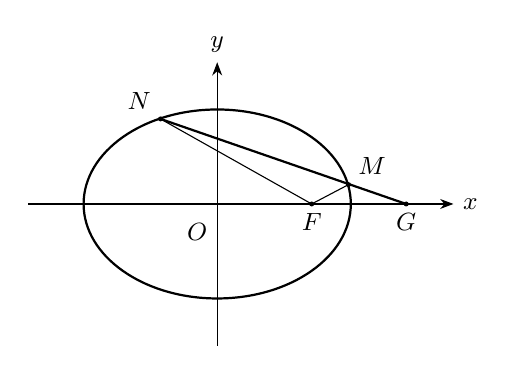
\begin{tikzpicture}[scale=0.6,>=Stealth,font=\small]
    % 坐标轴
    \draw[->] (-4,0) -- (5,0) node[right]{$x$};
    \draw[->] (0,-3) -- (0,3) node[above]{$y$};
    \node at (0,-0.2) [below left] {$O$};
    
    % 椭圆参数：a=2√2≈2.828，b=2
    \draw[thick] (0,0) ellipse (2.828 and 2);
    
    % 焦点F(2,0)、点G(4,0)
    \coordinate (F) at (2,0);
    \coordinate (G) at (4,0);
    \fill (F) circle (1.5pt) node[below] {$F$};
    \fill (G) circle (1.5pt) node[below] {$G$};
    
    % 核心修改：严格保证N、M、G三点共线
    % 先取直线GNM上的点N，再求直线与椭圆的另一个交点M
    \coordinate (N) at (-1.2,1.8); % N在椭圆上
    % 直线NG的参数方程，求与椭圆的另一个交点M
    \coordinate (M) at (2.78,0.41); % M在椭圆上，且N、M、G严格共线
    
    \fill (N) circle (1.5pt) node[above left] {$N$};
    \fill (M) circle (1.5pt) node[above right] {$M$};
    
    % 连线：N-M-G严格共线
    \draw[thick] (N) -- (G);
    \draw (N) -- (F);
    \draw (M) -- (F);
\end{tikzpicture}
\end{center}
\newpage


\subsection{圆锥曲线中的最值问题（大题）}

\textbf{例一： (2019天津一中月考)} 已知椭圆$C:\dfrac{x^2}{a^2}+\dfrac{y^2}{b^2}=1(a>b>0)$经过点$\left(1,\dfrac{\sqrt{3}}{2}\right)$，一个焦点为$(\sqrt{3},0)$。
\begin{enumerate}[label=(\Roman*)]
    \item 求椭圆$C$的方程；
    \item 若直线$y=k(x-1)(k\neq0)$与$x$轴交于点$P$，与椭圆$C$交于$A,B$两点，线段$AB$的垂直平分线与$x$轴交于点$Q$，求$\dfrac{|AB|}{|PQ|}$的取值范围。
\end{enumerate}

\vspace{18\baselineskip}

\textbf{例二： } 已知椭圆$\dfrac{x^2}{a^2}+\dfrac{y^2}{b^2}=1(a>b>0)$的离心率为$\dfrac{\sqrt{3}}{2}$，左、右顶点分别为$A,B$，上顶点为$D$，坐标原点$O$到直线$AD$的距离为$\dfrac{2\sqrt{5}}{5}$。
\begin{enumerate}[label=(\Roman*)]
    \item 求椭圆的方程；
    \item 过$A$点作两条互相垂直的直线$AP,AQ$与椭圆交于$P,Q$两点，求$\triangle BPQ$面积的最大值。
\end{enumerate}

\newpage

\textbf{例三： (2019全国二卷)} 已知点$A(-2,0)$，$B(2,0)$，动点$M(x,y)$满足直线$AM$与$BM$的斜率之积为$-\dfrac{1}{2}$。记$M$的轨迹为曲线$C$。
\begin{enumerate}[label=(\Roman*)]
    \item 求$C$的方程，并说明$C$是什么曲线。
    \item 过坐标原点的直线交$C$于$P,Q$两点，点$P$在第一象限，$PE \perp x$轴，垂足为$E$，连接$QE$并延长交$C$于点$G$。
    \begin{enumerate}[label=(\roman*)]
        \item 证明：$\triangle PQG$是直角三角形；
        \item 求$\triangle PQG$面积的最大值。
    \end{enumerate}
\end{enumerate}

\vspace{18\baselineskip}

\textbf{例四： (2020浙江)}已知椭圆$C_1:\dfrac{x^2}{2} + y^2 = 1$，抛物线$C_2:y^2 = 2px(p>0)$，点$A$是椭圆$C_1$与抛物线$C_2$的交点，过点$A$的直线$l$交椭圆$C_1$于点$B$，交抛物线$C_2$于点$M$（$B,M$不同于$A$）。
    \begin{enumerate}[label=(\arabic*)]
        \item 若$p = \dfrac{1}{16}$，求抛物线$C_2$的焦点坐标；
        \item 若存在不过原点的直线$l$使$M$为线段$AB$的中点，求$p$的最大值。
    \end{enumerate}

\newpage

\subsection{齐次化方法}

\textbf{例一： } 若直线$l$与椭圆$C:\dfrac{x^2}{4}+\dfrac{y^2}{3}=1$相交于$A$，$B$两点（$A$，$B$不是左、右顶点），且以$AB$为直径的圆过椭圆$C$的右顶点$D$。求证：直线$l$过定点，并求出该定点的坐标。

\vspace{18\baselineskip}

\textbf{例二： } 已知椭圆$C:\dfrac{x^2}{6}+\dfrac{y^2}{3}=1$过点$A(2,1)$。点$M$，$N$在$C$上，且$AM \perp AN$，$AD \perp MN$，$D$为垂足。证明：存在定点$Q$，使得$|DQ|$为定值。

\newpage

\section{综合练习}

\noindent\textbf{例一：} 若双曲线$C$的虚轴长为实轴长的$\sqrt{7}$倍，则$C$的离心率为
\vspace{0.5em}

A. $\sqrt{2}$ \quad B. $2$ \quad C. $\sqrt{7}$ \quad D. $2\sqrt{2}$
\vspace{3\baselineskip}

\noindent\textbf{例二：} 若圆$x^2+(y+2)^2=r^2(r>0)$上到直线$y=\sqrt{3}x+2$的距离为$1$的点有且仅有$2$个，则$r$的取值范围是
\vspace{0.5em}

A. $(0,1)$ \quad B. $(1,3)$ \quad C. $(3,+\infty)$ \quad D. $(0,+\infty)$
\vspace{3\baselineskip}

\noindent\textbf{例三：} 设抛物线$C:y^2=2px(p>0)$的焦点为$F$，点$A$在$C$上，过$A$作$C$准线的垂线，垂足为$B$。若直线$BF$的方程为$y=-2x+2$，则$|AF|=$
\vspace{0.5em}

A. $3$ \quad B. $4$ \quad C. $5$ \quad D. $6$
\vspace{3\baselineskip}

\noindent\textbf{例四：} (2024河东二模)双曲线$E:\dfrac{x^2}{a^2}-\dfrac{y^2}{b^2}=1(a>0,b>0)$的左、右焦点分别为$F_1,F_2$，$Q$为线段$F_1F_2$上一点，$P$为双曲线上第一象限内一点，$S_{\triangle PQF_1}=2S_{\triangle PQF_2}$，$\triangle PQF_1$与$\triangle PQF_2$的周长之和为$10a$，且它们的内切圆半径相等，则双曲线的离心率为
\vspace{0.5em}

A. $2$ \quad B. $4$ \quad C. $5$ \quad D. $6$
\vspace{3\baselineskip}

\noindent\textbf{例五：} (2022部分区二模)已知双曲线$C:\dfrac{x^2}{9}-\dfrac{y^2}{b^2}=1(b>0)$的左、右焦点分别为$F_1,F_2$，点$M$在$C$的左支上，过点$M$作$C$的一条渐近线的垂线，垂足为$N$，若$|MF_2|+|MN|$的最小值为$9$，则该双曲线的离心率为
\vspace{0.5em}

A. $\sqrt{2}$ \quad B. $\sqrt{3}$ \quad C. $\dfrac{3}{2}$ \quad D. $\dfrac{5}{3}$
\vspace{3\baselineskip}

\noindent\textbf{例六：} (2023十二校二模)抛物线$y^2=2ax(a>0)$上的点$M(x_0,3)$到其焦点的距离是$M$到$y$轴距离的$2$倍，过双曲线$C:\dfrac{x^2}{a^2}-\dfrac{y^2}{b^2}=1(a>0,b>0)$的左、右顶点$A,B$作双曲线$C$的同一条渐近线的垂线，垂足分别为$P,Q$，$|PQ|=4$，则双曲线的离心率为
\vspace{0.5em}

A. $\dfrac{\sqrt{5}}{2}$ \quad B. $\dfrac{\sqrt{14}}{3}$ \quad C. $\dfrac{\sqrt{5}}{3}$ \quad D. $\dfrac{3}{2}$
\newpage

% ==================== 大题部分 ====================
\noindent\textbf{例一：}(2025新高考一卷)设椭圆$C:\dfrac{x^2}{a^2}+\dfrac{y^2}{b^2}=1(a>b>0)$，椭圆的下顶点为$A$，右顶点为$B$，$|AB|=\sqrt{10}$，且椭圆$C$的离心率为$\dfrac{2\sqrt{2}}{3}$。
\vspace{0.5em}

(1) 求椭圆的标准方程；
\vspace{1\baselineskip}

(2) 已知动点$P$不在$y$轴上，动点$R$在射线$AP$上，且满足$|AR|\cdot|AP|=3$。
\vspace{0.5em}

(i) 设$P(m,n)$，求$R$的坐标（用$m,n$表示）；
\vspace{1\baselineskip}

(ii) 设$O$为坐标原点，$Q$是$C$上的动点，直线$OR$的斜率是直线$OP$的斜率的$3$倍，求$|PQ|$的最大值。
\vspace{20\baselineskip}

\noindent\textbf{例二：} (2022南开三模)已知焦点在$x$轴上，中心在原点，离心率为$\dfrac{\sqrt{3}}{2}$的椭圆经过点$M(2,1)$，动点$A,B$(不与点$M$重合)均在椭圆上，且直线$MA$与$MB$的斜率之和为$1$。
\vspace{0.5em}

(1) 求椭圆的方程；
\vspace{1\baselineskip}

(2) 证明直线$AB$经过定点，并求这个定点的坐标。
\vspace{2\baselineskip}






\end{document}
